%  LaTeX support: latex@mdpi.com 
%  For support, please attach all files needed for compiling as well as the log file, and specify your operating system, LaTeX version, and LaTeX editor.

%=================================================================
\documentclass[energies,article,accept,pdftex,moreauthors]{Definitions/mdpi} 

%--------------------
% Class Options:
%--------------------
%----------
% journal
%----------
% Choose between the following MDPI journals:
% acoustics, actuators, addictions, admsci, adolescents, aerobiology, aerospace, agriculture, agriengineering, agrochemicals, agronomy, ai, air, algorithms, allergies, alloys, analytica, analytics, anatomia, animals, antibiotics, antibodies, antioxidants, applbiosci, appliedchem, appliedmath, applmech, applmicrobiol, applnano, applsci, aquacj, architecture, arm, arthropoda, arts, asc, asi, astronomy, atmosphere, atoms, audiolres, automation, axioms, bacteria, batteries, bdcc, behavsci, beverages, biochem, bioengineering, biologics, biology, biomass, biomechanics, biomed, biomedicines, biomedinformatics, biomimetics, biomolecules, biophysica, biosensors, biotech, birds, bloods, blsf, brainsci, breath, buildings, businesses, cancers, carbon, cardiogenetics, catalysts, cells, ceramics, challenges, chemengineering, chemistry, chemosensors, chemproc, children, chips, cimb, civileng, cleantechnol, climate, clinpract, clockssleep, cmd, coasts, coatings, colloids, colorants, commodities, compounds, computation, computers, condensedmatter, conservation, constrmater, cosmetics, covid, crops, cryptography, crystals, csmf, ctn, curroncol, cyber, dairy, data, ddc, dentistry, dermato, dermatopathology, designs, devices, diabetology, diagnostics, dietetics, digital, disabilities, diseases, diversity, dna, drones, dynamics, earth, ebj, ecologies, econometrics, economies, education, ejihpe, electricity, electrochem, electronicmat, electronics, encyclopedia, endocrines, energies, eng, engproc, entomology, entropy, environments, environsciproc, epidemiologia, epigenomes, est, fermentation, fibers, fintech, fire, fishes, fluids, foods, forecasting, forensicsci, forests, foundations, fractalfract, fuels, future, futureinternet, futurepharmacol, futurephys, futuretransp, galaxies, games, gases, gastroent, gastrointestdisord, gels, genealogy, genes, geographies, geohazards, geomatics, geosciences, geotechnics, geriatrics, grasses, gucdd, hazardousmatters, healthcare, hearts, hemato, hematolrep, heritage, higheredu, highthroughput, histories, horticulturae, hospitals, humanities, humans, hydrobiology, hydrogen, hydrology, hygiene, idr, ijerph, ijfs, ijgi, ijms, ijns, ijpb, ijtm, ijtpp, ime, immuno, informatics, information, infrastructures, inorganics, insects, instruments, inventions, iot, j, jal, jcdd, jcm, jcp, jcs, jcto, jdb, jeta, jfb, jfmk, jimaging, jintelligence, jlpea, jmmp, jmp, jmse, jne, jnt, jof, joitmc, jor, journalmedia, jox, jpm, jrfm, jsan, jtaer, jvd, jzbg, kidneydial, kinasesphosphatases, knowledge, land, languages, laws, life, liquids, literature, livers, logics, logistics, lubricants, lymphatics, machines, macromol, magnetism, magnetochemistry, make, marinedrugs, materials, materproc, mathematics, mca, measurements, medicina, medicines, medsci, membranes, merits, metabolites, metals, meteorology, methane, metrology, micro, microarrays, microbiolres, micromachines, microorganisms, microplastics, minerals, mining, modelling, molbank, molecules, mps, msf, mti, muscles, nanoenergyadv, nanomanufacturing,\gdef\@continuouspages{yes}} nanomaterials, ncrna, ndt, network, neuroglia, neurolint, neurosci, nitrogen, notspecified, %%nri, nursrep, nutraceuticals, nutrients, obesities, oceans, ohbm, onco, %oncopathology, optics, oral, organics, organoids, osteology, oxygen, parasites, parasitologia, particles, pathogens, pathophysiology, pediatrrep, pharmaceuticals, pharmaceutics, pharmacoepidemiology,\gdef\@ISSN{2813-0618}\gdef\@continuous pharmacy, philosophies, photochem, photonics, phycology, physchem, physics, physiologia, plants, plasma, platforms, pollutants, polymers, polysaccharides, poultry, powders, preprints, proceedings, processes, prosthesis, proteomes, psf, psych, psychiatryint, psychoactives, publications, quantumrep, quaternary, qubs, radiation, reactions, receptors, recycling, regeneration, religions, remotesensing, reports, reprodmed, resources, rheumato, risks, robotics, ruminants, safety, sci, scipharm, sclerosis, seeds, sensors, separations, sexes, signals, sinusitis, skins, smartcities, sna, societies, socsci, software, soilsystems, solar, solids, spectroscj, sports, standards, stats, std, stresses, surfaces, surgeries, suschem, sustainability, symmetry, synbio, systems, targets, taxonomy, technologies, telecom, test, textiles, thalassrep, thermo, tomography, tourismhosp, toxics, toxins, transplantology, transportation, traumacare, traumas, tropicalmed, universe, urbansci, uro, vaccines, vehicles, venereology, vetsci, vibration, virtualworlds, viruses, vision, waste, water, wem, wevj, wind, women, world, youth, zoonoticdis 
% For posting an early version of this manuscript as a preprint, you may use "preprints" as the journal. Changing "submit" to "accept" before posting will remove line numbers.

%---------
% article
%---------
% The default type of manuscript is "article", but can be replaced by: 
% abstract, addendum, article, book, bookreview, briefreport, casereport, comment, commentary, communication, conferenceproceedings, correction, conferencereport, entry, expressionofconcern, extendedabstract, datadescriptor, editorial, essay, erratum, hypothesis, interestingimage, obituary, opinion, projectreport, reply, retraction, review, perspective, protocol, shortnote, studyprotocol, systematicreview, supfile, technicalnote, viewpoint, guidelines, registeredreport, tutorial
% supfile = supplementary materials

%----------
% submit
%----------
% The class option "submit" will be changed to "accept" by the Editorial Office when the paper is accepted. This will only make changes to the frontpage (e.g., the logo of the journal will get visible), the headings, and the copyright information. Also, line numbering will be removed. Journal info and pagination for accepted papers will also be assigned by the Editorial Office.

%------------------
% moreauthors
%------------------
% If there is only one author the class option oneauthor should be used. Otherwise use the class option moreauthors.

%---------
% pdftex
%---------
% The option pdftex is for use with pdfLaTeX. Remove "pdftex" for (1) compiling with LaTeX & dvi2pdf (if eps figures are used) or for (2) compiling with XeLaTeX.

%=================================================================
% MDPI internal commands - do not modify
\firstpage{1} 
\makeatletter 
\setcounter{page}{\@firstpage} 
\makeatother
\pubvolume{1}
\issuenum{1}
\articlenumber{0}
\pubyear{2023}
\copyrightyear{2023}
\externaleditor{Academic Editor: Abu-Siada\linebreak Ahmed}
\datereceived{28 July 2023} 
\daterevised{17 August 2023} % Comment out if no revised date
\dateaccepted{18 August 2023} 
\datepublished{ } 
%\datecorrected{} % For corrected papers: "Corrected: XXX" date in the original paper.
%\dateretracted{} % For corrected papers: "Retracted: XXX" date in the original paper.
\hreflink{https://doi.org/} % If needed use \linebreak
%\doinum{}
%\pdfoutput=1 % Uncommented for upload to arXiv.org

%=================================================================
% Add packages and commands here. The following packages are loaded in our class file: fontenc, inputenc, calc, indentfirst, fancyhdr, graphicx, epstopdf, lastpage, ifthen, float, amsmath, amssymb, lineno, setspace, enumitem, mathpazo, booktabs, titlesec, etoolbox, tabto, xcolor, colortbl, soul, multirow, microtype, tikz, totcount, changepage, attrib, upgreek, array, tabularx, pbox, ragged2e, tocloft, marginnote, marginfix, enotez, amsthm, natbib, hyperref, cleveref, scrextend, url, geometry, newfloat, caption, draftwatermark, seqsplit
% cleveref: load \crefname definitions after \begin{document}
\usepackage[labelformat=simple]{subcaption}
\renewcommand\thesubfigure{\alph{subfigure}}
\DeclareCaptionLabelFormat{subcaptionlabel}{\normalfont(\textbf{#2}\normalfont)}
\captionsetup[subfigure]{labelformat=subcaptionlabel}

\usepackage{comment}

%=================================================================
% Please use the following mathematics environments: Theorem, Lemma, Corollary, Proposition, Characterization, Property, Problem, Example, ExamplesandDefinitions, Hypothesis, Remark, Definition, Notation, Assumption
%% For proofs, please use the proof environment (the amsthm package is loaded by the MDPI class).

%=================================================================
% Full title of the paper (Capitalized)
\Title{Neural Network Architecture for
Determining the Aging of Stationary
Storage Systems in Smart Grids}

% MDPI internal command: Title for citation in the left column
\TitleCitation{Neural Network Architecture for
Determining the Aging of Stationary
Storage Systems in Smart Grids}

% Author Orchid ID: enter ID or remove command
\newcommand{\orcidauthorA}{0000-0000-0000-000X} % Add \orcidA{} behind the author's name
%\newcommand{\orcidauthorB}{0000-0000-0000-000X} % Add \orcidB{} behind the author's name

% Authors, for the paper (add full first names)
\Author{\hl{Florian Rzepka} *$^{,\dagger}$, Philipp Hematty $^{\dagger}$, Mano Schmitz and Julia Kowal *}
%MDPI: Please carefully check the accuracy of names and affiliations.


% MDPI internal command: Authors, for metadata in PDF
\AuthorNames{Florian Rzepka, Philipp Hematty, Mano Schmitz and Julia Kowal}

% MDPI internal command: Authors, for citation in the left column
\AuthorCitation{\hl{Rzepka}, F.; Hematty, P.; Schmitz, M; Kowal, F.}
%MDPI: Please check all author names carefully.

\address[1]{%
TU Berlin, Electrical Energy Storage Technology, Einsteinufer 11, D-10587 Berlin, \hl{Germany}; %MDPI: Country added, please confirm.    
%MDPI: The Current address in the note can NOT be same with the affiliation. We removed the current address. Please confirm.
\linebreak \hl{p.hematty@campus.tu-berlin.de (P.H.); m.schmitz@tu-berlin.de (M.S.)}}%MDPI: We added the email addresses here according to those submitted online at susy.mdpi.com. Please confirm.
\corres{\hangafter=1 \hangindent=1.05em \hspace{-0.82em}Correspondence: florian.rzepka@tu-berlin.de (F.R.); julia.kowal@tu-berlin.de (J.K.)}




% Current address and/or shared authorship
\firstnote{\hangafter=1 \hangindent=1.05em \hspace{-0.82em} \hl{These} authors contributed equally to this work.} 
%MDPI: The Current address in the note can NOT be same with the affiliation. So we removed it and revised the symbol of the first note. Please confirm.


%\secondnote{\hangafter=1 \hangindent=1.05em \hspace{-0.82em} }
% The commands \thirdnote{} till \eighthnote{} are available for further notes

%\simplesumm{} % Simple summary

%\conference{} % An extended version of a conference paper

% Abstract (Do not insert blank lines, i.e. \\) 
\abstract{The estimation of the State-of-Health (SOH) of energy storage systems is a key task to ensure their reliable operation and maintenance. This paper investigates a new SOH determination method for stationary storage in Microgrids. Aging tests are conducted on NMC cells, with test profiles corresponding to Microgrids' conditions. The focus of this work is on optimizing the learning process and the application of a Multilayer Perceptron (MLP) model to address this issue. This study introduces a novel approach of considering lag sequences, or time series data, to expedite the learning procedure and enhance prediction accuracy.
A key advancement in this research is the usage of shorter time intervals to calculate the SOH, which not only reduces the learning time but also decreases the application time. This approach led to an overall reduction in computational effort when estimating the SOH.
Energy is introduced as a new input parameter, resulting in improved modeling and more accurate SOH estimations. Furthermore, the MLP model achieved a Mean Squared Error (MSE) of 2.95 and a Mean Absolute Error (MAE) of 1.10, which are indicative of its strong predictive accuracy.
Emphasis was also placed on the careful tuning and optimization of the neural network's hyperparameters. The goal was to design a computationally efficient network that still yields optimal results. The findings demonstrate the effectiveness and potential of the MLP model in SOH estimation, underscoring the importance of the methodical model design and hyperparameter optimization.} %v3.0

% Keywords
\keyword{State-of-Health (SOH) estimation; Multilayer Perceptron (MLP) model; lag sequences} 

% The fields PACS, MSC, and JEL may be left empty or commented out if not applicable
%\PACS{J0101}
%\MSC{}
%\JEL{}

%%%%%%%%%%%%%%%%%%%%%%%%%%%%%%%%%%%%%%%%%%
% Only for the journal Diversity
%\LSID{\url{http://}}

%%%%%%%%%%%%%%%%%%%%%%%%%%%%%%%%%%%%%%%%%%
% Only for the journal Applied Sciences
%\featuredapplication{Authors are encouraged to provide a concise description of the specific application or a potential application of the work. This section is not mandatory.}
%%%%%%%%%%%%%%%%%%%%%%%%%%%%%%%%%%%%%%%%%%

%%%%%%%%%%%%%%%%%%%%%%%%%%%%%%%%%%%%%%%%%%
% Only for the journal Data
%\dataset{DOI number or link to the deposited data set if the data set is published separately. If the data set shall be published as a supplement to this paper, this field will be filled by the journal editors. In this case, please submit the data set as a supplement.}
%\datasetlicense{License under which the data set is made available (CC0, CC-BY, CC-BY-SA, CC-BY-NC, etc.)}

%%%%%%%%%%%%%%%%%%%%%%%%%%%%%%%%%%%%%%%%%%
% Only for the journal Toxins
%\keycontribution{The breakthroughs or highlights of the manuscript. Authors can write one or two sentences to describe the most important part of the paper.}

%%%%%%%%%%%%%%%%%%%%%%%%%%%%%%%%%%%%%%%%%%
% Only for the journal Encyclopedia
%\encyclopediadef{For entry manuscripts only: please provide a brief overview of the entry title instead of an abstract.}

%%%%%%%%%%%%%%%%%%%%%%%%%%%%%%%%%%%%%%%%%%
% Only for the journal Advances in Respiratory Medicine
%\addhighlights{yes}
%\renewcommand{\addhighlights}{%

%\noindent This is an obligatory section in “Advances in Respiratory Medicine”, whose goal is to increase the discoverability and readability of the article via search engines and other scholars. Highlights should not be a copy of the abstract, but a simple text allowing the reader to quickly and simplified find out what the article is about and what can be cited from it. Each of these parts should be devoted up to 2~bullet points.\vspace{3pt}\\
%\textbf{What are the main findings?}
% \begin{itemize}[labelsep=2.5mm,topsep=-3pt]
% \item First bullet.
% \item Second bullet.
% \end{itemize}\vspace{3pt}
%\textbf{What is the implication of the main finding?}
% \begin{itemize}[labelsep=2.5mm,topsep=-3pt]
% \item First bullet.
% \item Second bullet.
% \end{itemize}
%}

%%%%%%%%%%%%%%%%%%%%%%%%%%%%%%%%%%%%%%%%%%
\begin{document}

%%%%%%%%%%%%%%%%%%%%%%%%%%%%%%%%%%%%%%%%%%
\section{Introduction}

Estimating State-of-Health (SOH) is a crucial aspect of ensuring the reliable operation and maintenance of energy storage systems, particularly in the context of microgrids. The challenge of energy management in microgrids has been highlighted in previous studies \cite{Sahri.2021, Soliman.2021}. In the context of these complex systems, we recognize the SOH of batteries as a vital parameter, as it plays a crucial role in maintaining reliability and efficiency. Accurate SOH estimation can significantly contribute to the effective management of the system, optimizing power usage, reducing costs, and maximizing performance. This is especially relevant in the complex landscape of microgrid energy management, where the integration of renewable sources and the need for resilience against fluctuations require precise monitoring and control. Two approaches have been used to estimate the SOH: the model-based and data-driven approach \cite{Gou.2020}. While model-based approaches rely on physics-based models of the system, data-driven approaches utilize machine learning algorithms to learn the relationships between the input and output data. %v3.0 

In general, data-driven approaches rely on measured input-output data, while model-based approaches require a detailed understanding of the system's underlying physics. While model-based approaches can provide accurate results under ideal conditions, they can be limited by the simplifying assumptions made in the model and can be computationally expensive to solve. In contrast, data-driven approaches can handle complex and non-linear relationships between input and output data, making them more versatile and efficient for SOH estimation. Furthermore, data-driven approaches do not require the same level of knowledge of the system as model-based approaches, making them more accessible for practical applications \cite{Oji.2021}.

%% Smart Grid Context
In the context of smart grids, the proposed method's applicability extends beyond traditional energy storage systems. Smart grids are complex networks that integrate various energy sources, storage systems, and consumption patterns. The test system used in this study is designed to emulate the dynamic and multifaceted nature of smart grids. Through laboratory tests with cells under various conditions representative of those encountered in smart grids, a realistic platform was created. The use of a Multilayer Perceptron (MLP) for evaluating the State-of-Health (SOH) further contributes to the test system's alignment with real-world applications. This comprehensive approach ensures that the findings are directly translatable to real-world smart grid scenarios, enhancing the method's practical value. %v.3.0%

%% Model based
Li et al. propose a method using a dual Kalman filter and the forgetting factor recursive least squares (FFRLS) method for the SOC and SOH estimation of LIBs, with errors within 1\%. However, this method has limitations, including sensitivity to the accuracy of the OCV-SOC curve and cell capacity, reliance on precise model parameter identification, and potential influence by the initial SOC \cite{Li.2021}.

Bi et al. utilize a physics-based model and a particle filter to address capacity and power degradation, predicting aging parameters and failure with estimation errors within 3\% for capacity fade and 4\% for power fade. Despite its innovation, this method faces challenges such as a difficulty in generalizing an empirical relationship between aging parameters and cell degradation rate, need for filter tuning, particle degeneracy problem, need for equation simplification for real-time applications, and potential computational time constraint \cite{Bi.2020}.

Tian et al. focus on SOH estimation and aging mechanism identification using a Fractional Order Model (FOM), estimating the remaining capacity with an error within 3.1\%. This method, however, has challenges such as the inability to distinguish between different aging mechanisms, computational burden when using the electrochemical model, insensitivity to the discharge rate of aging cycle tests, and requirement for offline operations and specific parameter identification methods \cite{Tian.2019}.

%% data driven
In the field of data-driven approaches, methods can be categorized into those based on machine learning and those reliant on direct measurement. Ebert et al. propose a direct measurement method utilizing a single pressure sensor to detect abnormal behavior in lithium-ion battery cells, such as capacity fade and mechanical failure. However, this method faces challenges in differentiating failure modes and requires detailed reference measurements, potentially limiting its practical use \cite{Ebert.2017}.

Stroe et al. present another direct measurement method that estimates the capacity fade by considering a reduced voltage interval. Despite showing promising results with an average error below 2.5\%, this method may yield increased estimation errors at higher degradation levels due to changes in the selected voltage interval \cite{Stroe.2018b}.

In a separate study, Stroe et al. explore the Incremental Capacity Analysis (ICA) technique for estimating the state-of-health (SOH) of LMO/NMC-based Lithium-ion cells. However, this method is sensitive to changes in charging conditions and may underestimate the capacity fade, especially at higher degradation levels \cite{Stroe.2018}.

%% machine learning
Shifting the focus to machine learning methods, Shi et al. offer a significant contribution with their hybrid method for SOH estimation that combines advanced Kalman filters and deep neural networks, reducing estimation errors to 2\% \cite{Shi.2021}. However, this method is constrained by the complexity and time-consuming nature of tuning and optimizing the Fully Connected Deep Network (FCDN) model used for SOC estimation.

Kim et al. propose the ARIMA model, which harnesses historical cell data for future state predictions, but struggles with less accurate long-term predictions due to its inability to consider external factors. Furthermore, artificial intelligence models used for predicting lithium-ion cells' State of Health (SOH) can be complex, lack interpretability, and are often limited to a single variable \cite{Kim.2022}.

Xiong et al. introduce a different approach with an online SOH estimation method for retired lithium-ion cells, leveraging a weighted least squares support vector machine (WLS-SVM). While it is superior to popular methods such as the Backpropagation Neural Network (BPNN) and SVM, it can display an increased error rate with abnormal training points in the data \cite{Xiong.2021}.

Sui's approach uses the fuzzy entropy (FE) of voltage as a feature for SOH estimation with support vector machines (SVM). Despite its high accuracy, it requires extensive laboratory testing, and some features might lose validity under different conditions such as temperature variations or changes in the state of charge (SOC) \cite{Sui.}.

Jo et al. propose a novel data preprocessing method that uses a relative state of charge (SOC) to enhance machine learning efficiency for SOH estimation. This method, while innovative, could be compromised by errors in calculating or determining the relative SOC~\cite{Jo.2021}.

%% Hybrid Physics-Based and Data-Driven Approaches
Hybrid methods that combine physics-based and data-driven approaches are emerging as powerful tools for predicting the Li-Ion battery degradation. Two recent studies by Le Xu et al. \cite{LeXu.2023} and Hui Pang et al. \cite{Pang.2023} exemplify this trend, employing innovative techniques to enhance prediction accuracy and robustness. Specifically, the method proposed by Le Xu et al. consists of hybrid feature extraction, clustering, and prediction using a sequence-to-sequence deep learning framework. With only 20\% data, this approach achieves mean absolute percentage errors (MEPAEs) below 2.5\% for the capacity trajectory and 6.5\% for the remaining useable cycles. When 50\% of data are used, the MEPAEs are further reduced to less than 1.3\% and 5\%. However, the method's potential drawbacks could include its computational intensity, possibly limiting scalability, and concerns about generalizability across different battery types or conditions \cite{LeXu.2023}. %v3.0

Lastly, Kim et al. and Chaoui et al. present methods that feed raw parameters such as voltage, current, and temperature directly into the model for real-time SOH \mbox{estimation \cite{Kim.2018, Chaoui.2017}}. The potential pitfall of these approaches lies in the potential lack of contextual information, possibly omitting important insights into the battery health derived from these parameters' rate of change over time or their interactions.

%% Selection of MLP
In light of the above, while significant advancements have been made in the field of SOH estimation, each approach exhibits certain limitations, such as data dependency, complexity, the need for precise tuning, and the lack of robustness against imperfect data. Multi-Layer Perceptrons (MLP) offer a solution to these challenges by providing a flexibility in architecture, optimized weight estimation, and adaptability in capturing complex patterns. Their proven accuracy in various studies further justifies their application in SOH estimation \cite{Makridakis.2018}. %v.3.0

Having highlighted the challenges and proposed improvements in the preceding discussion, the following sections of this paper delve into the merits of neural networks, specifically Multilayer Perceptrons (MLP). This choice is motivated by their flexibility and power in capturing complex patterns and relationships that cannot be easily modelled~\cite{How.2019}. These methods can be implemented easily without requiring information on the electrochemical characteristics of battery cells and the environmental factors \cite{HossainLipu.2020}. The use of MLPs is further supported by their ability to provide accurate forecasts, adapt to various data scales, and offer computational efficiency, as evidenced in recent studies \cite{Makridakis.2018}. %v.3.0

%% Novelty and Advantages
The novelty of this work lies in the way data are preprocessed to provide a good estimation with a fairly simple neural network. It is a mixture of already known methods and the verification of their application for this field. What sets this approach apart is its comprehensive consideration of various parameters, including the strategic inclusion of energy as an input parameter, and the use of lag sequences to train the neural network. This method enhances the speed and efficiency of the training process, reduces the need for data storage, and offers a versatile and efficient solution. What is particularly advantageous about the method is that it can be generalizable to a large range of battery storage systems, regardless of scale and chemistry, assuming that there are enough data for training. Unlike traditional methods that may be constrained by specific charging patterns or require extensive laboratory testing, the proposed method's ability to handle imperfect data, adapt to various cell types and chemistries, and align with the dynamic nature of smart grids sets it apart from existing approaches. %v.3.0%

%% Purpose and Comparison with Simpler Controllers
This work aims to present a more comprehensive and resilient approach for estimating the State-of-Health (SOH) of lithium-ion cells, focusing on stationary energy storage in smart grids. While simpler controllers might offer solutions for specific scenarios, they often lack the flexibility and robustness required for complex and variable operating conditions such as those encountered in smart grids. The proposed method's adaptability and precision make it a valuable tool for enhancing energy storage management. %v.3.0%

Traditional methods for SOH estimation, such as capacity measurement, often become impractical in systems that are continuously in operation and do not exhibit clear charging patterns. As such, the method needs to determine the SOH from undefined states. The approach is designed to confront the specific challenges of such systems and improve upon the weaknesses identified in previous studies. For this purpose, measurements were conducted on NMC cells aged under various conditions---including different discharge currents, varying Depths of Discharge (DODs), and average States of Charge (SOCs).

Data segmentation is foundational to the methodology. The data are divided into individual parts using lag sequences to train the neural network. This allows the network to learn data flexibly, without needing specific patterns, such as a capacity measurement. This method enhances the speed and efficiency of the training process and reduces the need for data storage---a critical aspect for real-time applications.

Furthermore, the approach expands the range of inputs used for SOH estimation beyond the typically used current, voltage, and temperature. In particular, using energy as an additional input parameter is suggested. This comprehensive consideration of various parameters enables a robust and precise SOH estimation capable of handling outliers and imperfect data---a crucial requirement for practical applications.

An additional benefit of this work lies in its broad applicability. The method can be employed for other cell types, different capacity sizes, and various cell chemistries, even though only NMC cells were tested in this study. This promises a widespread application in various contexts and approaches, as it is a flexible and universal tool for SOH estimation. %Please verify.

Building on the context and challenges previously discussed, the structure of this research is subsequently outlined. This includes the unprocessed cell dataset, preprocessing methods, the structure of the neural network, experiment results, and the conclusion. The diagram in Figure \ref{process} provides a detailed representation of the workflow and the interrelationships among various steps in this study.

\begin{figure}[H]
%\centering
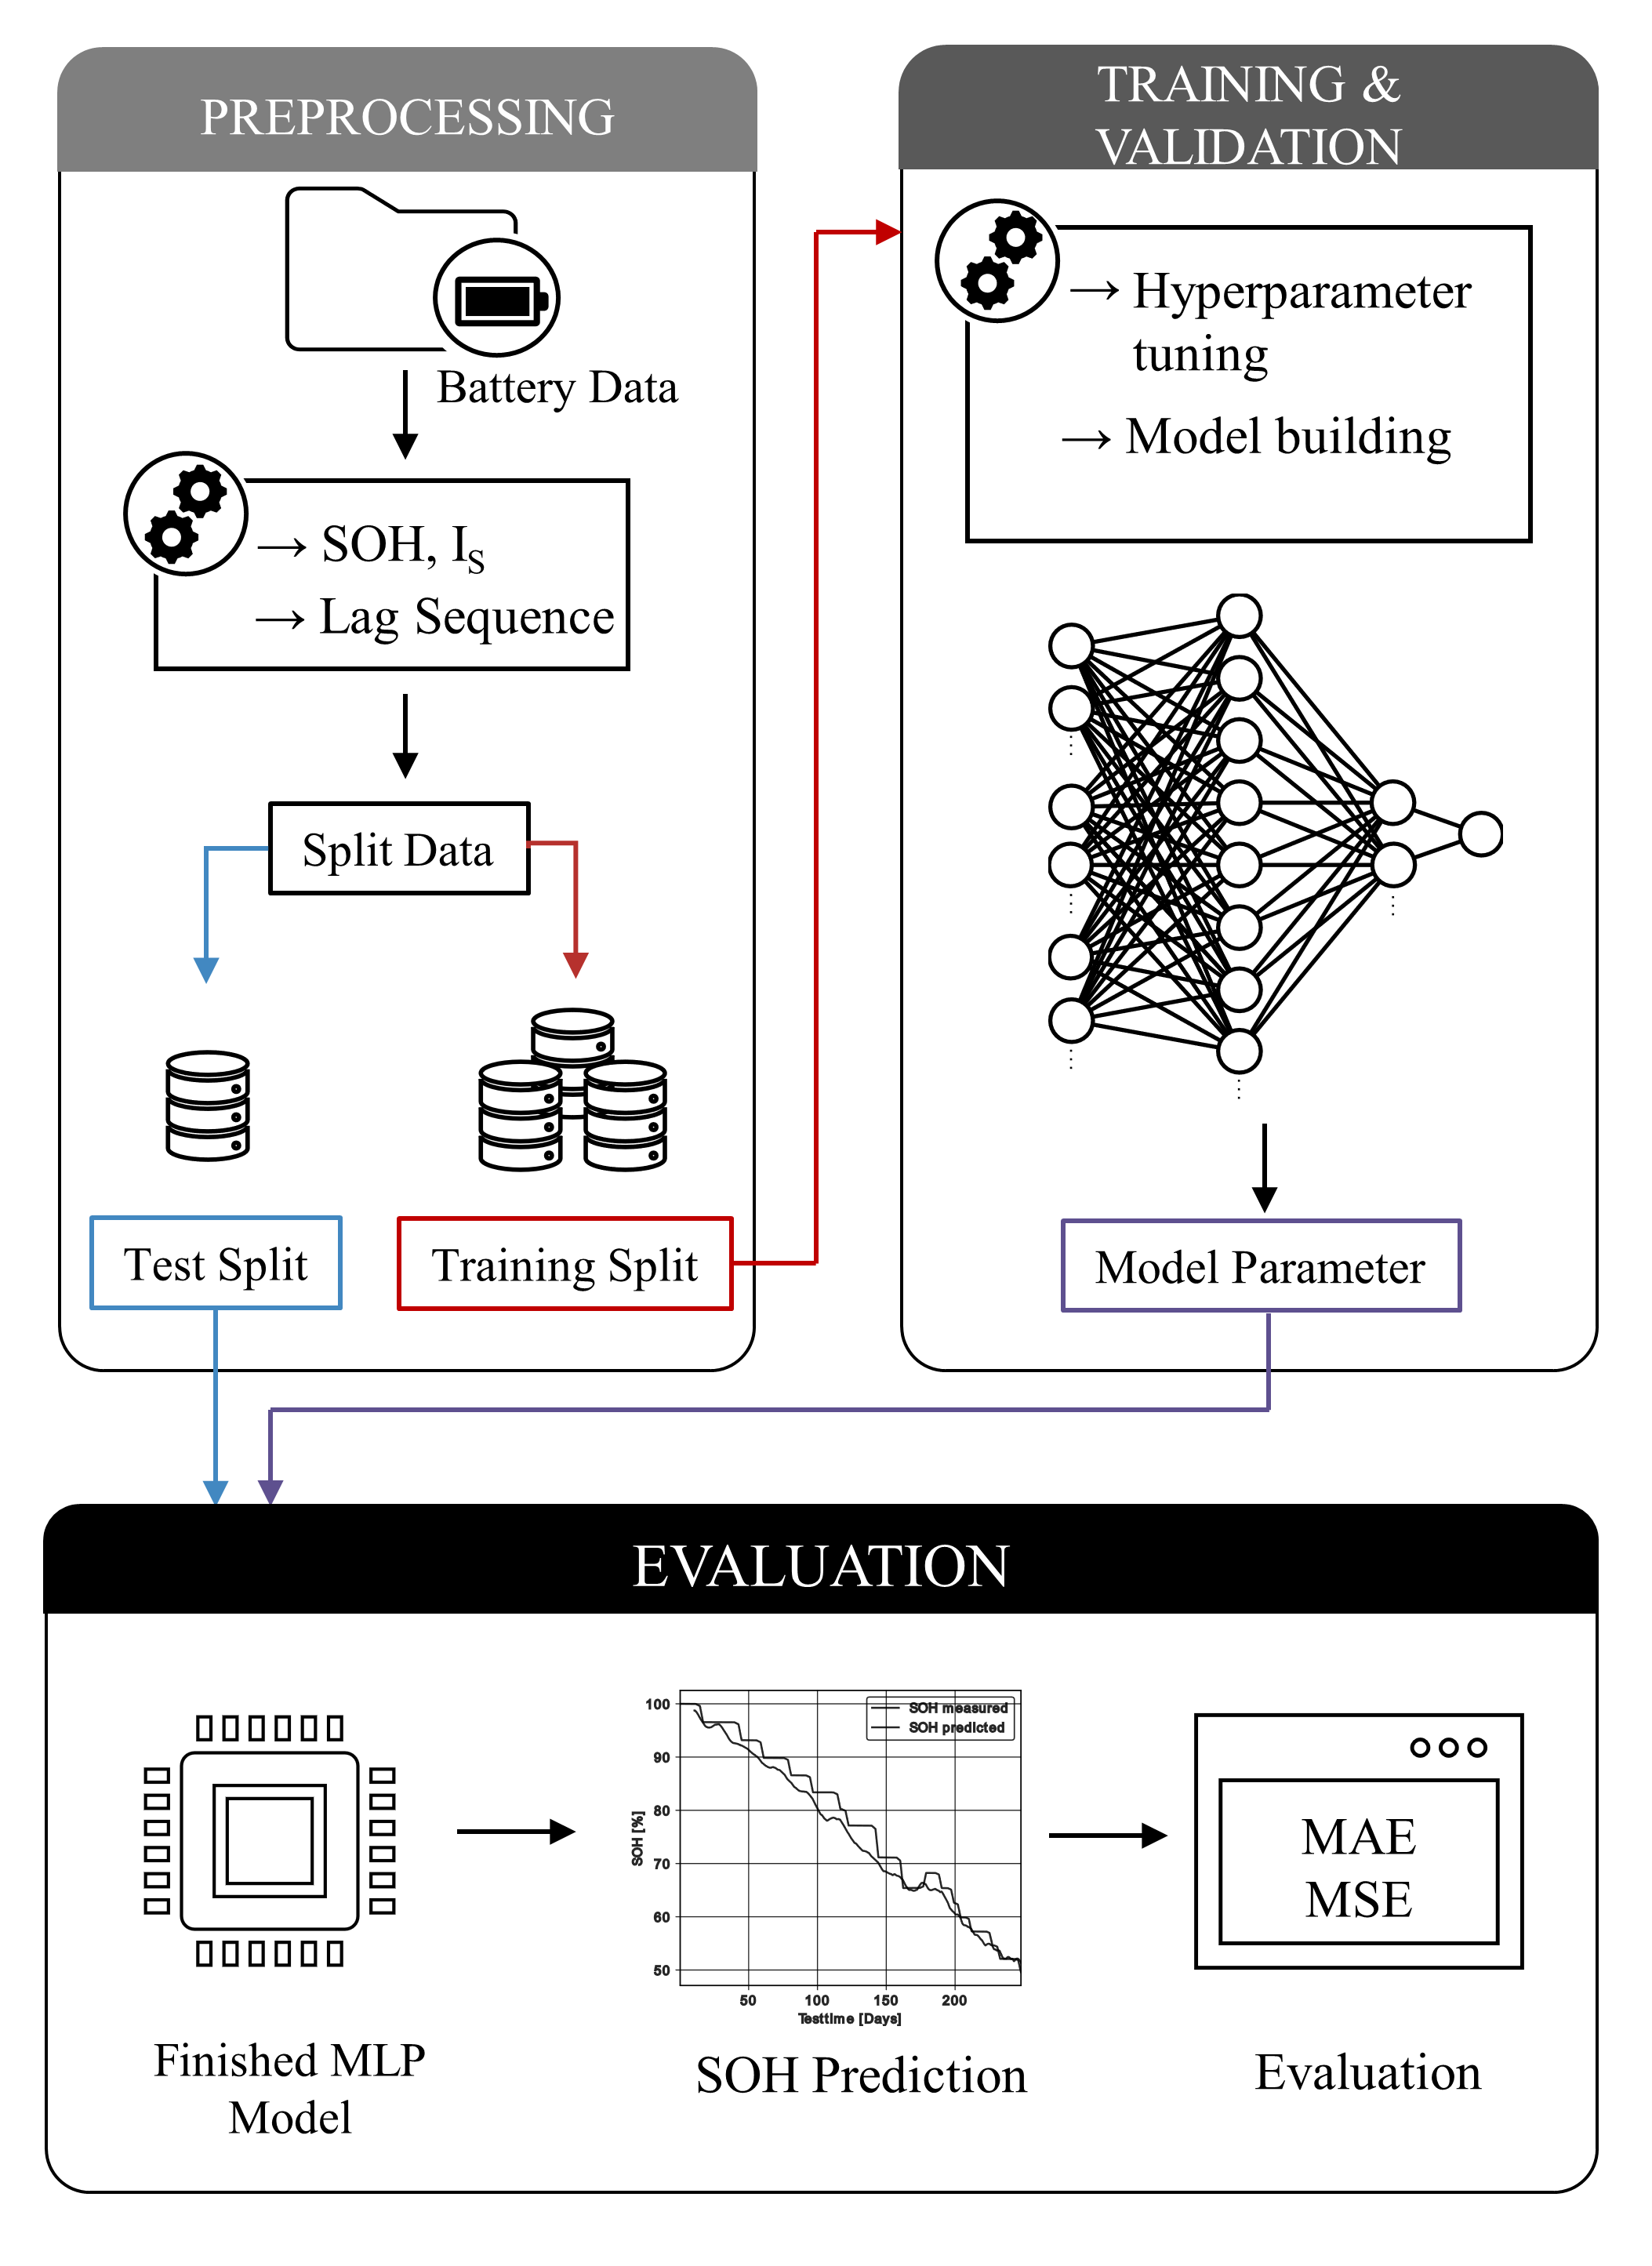
\includegraphics[width=9cm]{Figures/Process2.png}
\caption{\hl{The} %MDPI: The two lines of `SOH measured' and `SOH perdlcted' in the middle of the lower part of the picture seem to be similar. Please confirm whether they need to be modified and differentiated more clearly.
diagram outlines the stages of work from preprocessing raw cell data and training the neural network to evaluate the results. This representation provides insight into the data analysis, model building, and result assessment process.\label{process}}
\end{figure}

%%%%%%%%%%%%%%%%%%%%%%%%%%%%%%%%%%%%%%%%%%
\section{Raw Cell Dataset, Parameters and Measured Quantities}

This study employs data derived from an aging test conducted on Lithium-Ion cells, or, more specifically, NMC-type cells. %Please verify.
 The tested cells are Li-ion INR18650 cells with a capacity of 2600 mAh. These cells operate under a nominal voltage of 3.7 V, with a maximum charging voltage set to 4.2 V. The cut-off voltage for discharging these cells has been fixed at 2.75 V, and the maximum continuous discharge current allowed is 5.0 C. These cells are selected for the application and will later be used to build the battery pack. The smart grid system aims to connect multiple storage units, making the state determination, particularly the aging of the storage, crucial. All units must remain in a homogeneous state over time.

The aging tests on these cells were carried out at the Technical University of Berlin. The procedure involved cyclic aging tests at different temperatures and Depth of Discharge (DOD) levels. These parameters, including the temperatures, DOD, and C-rates used, are particularly applicable to stationary storage systems. The C-rates represent different discharge and charge currents, exposing the cells to varying power levels. Unlike mobile applications that experience high power surges, stationary storage systems in smart grids typically operate at lower C-rates, maintaining a less dynamic profile and avoiding sudden peaks. This approach aligns with the findings in \cite{Kucevic.2020}, where the standard profiles for stationary energy storage systems were analyzed. Furthermore, the mean State of Charge (SOC$_{mean}$) levels chosen reflect the usage patterns in stationary storage, where the cells often cycle around a specific point rather than being fully charged and discharged. This is largely due to the variable availability of renewable energy in smart grids, and the operating scenarios are defined based on the holistic simulation framework presented in~\cite{Kucevic.2020}. %v.3.0%

The cells underwent continuous charge and discharge cycles. For charging, the Constant Current Constant Voltage (CCCV) method was employed, whereas a constant current was used for discharging. The aging test comprised a specific number of cycles, followed by a capacity test to determine the capacity loss experienced by the cells. It is important to note that these aging and cycle tests comply with standard test methods \cite{Kassem.2012}. The primary aim of these tests was to study the targeted aging of the cells under certain conditions, and the charging and discharging scenarios were designed to reflect real-world applications in smart grids operating with various sources of electricity generation, including renewables.

The measurements obtained from these tests include the instantaneous value of the current flow, the cell voltage, and the time intervals during which the measurements were carried out. These time intervals varied depending on the process step and were resampled to 1 s.

Table \ref{scenario_params} illustrates seven distinct scenarios under which the cells aged. For each scenario, two cells were examined in detail. In total, 14 cells were utilized in this experiment, all of which were fresh and, thus, had a State of Health (\textit{SOH}) of 100\% at the initiation of the test. The scenarios vary based on four modifiable parameters: the State of Charge (SOC), the Depth of Discharge (DOD), the C-rate during discharge, and the operating temperature. These parameters were systematically varied to investigate their impacts on the aging process of the cells. The evaluation of these scenarios is crucial to understand the effect of different operational conditions on the life span and performance of the cells. An in-depth understanding of these factors will help optimize cell usage and design more efficient and durable energy storage systems.


\begin{table}[H] %MDPI: Table moved after first citation, please confirm.
\caption{\hl{The} test parameters were configured as follows: The charge was set at 1C, while the discharge was established at 1C and 2C. The capacity of the cells was 2.6 Ah, with a voltage cutoff delineated at 2.75 V and 4.2 V. The mean state of charge (\textit{SOC$_{mean}$}) was arranged at three distinct levels: 20\%, 50\%, and 80\%. The depth of discharge (\textit{DOD}) was evaluated at two stages: 30\% and 100\%. The investigation was carried out at two different temperatures: 35 °C and 45 °C.} 
\label{scenario_params}
\newcolumntype{C}{>{\centering\arraybackslash}X}
\begin{tabularx}{\textwidth}{CCCCCC}

\toprule
\textbf{Scenario} & \textbf{Cell No.} & \textbf{SOC$_{mean}$} & \textbf{DOD} & \textbf{C-Rate$_{dis}$} & \textbf{T ($^{\circ}$C)} \\
\midrule
1 & 1 and 2 & 50\% & 100\% & 1C & 35 \\
2 & 3 and 4 & 20\% & 30\% & 1C & 35 \\
3 & 5 and 6 & 50\% & 30\% & 1C & 35 \\
4 & 7 and 8 & 80\% & 30\% & 1C & 35 \\
5 & 9 and 10 & 50\% & 100\% & 2C & 35 \\
6 & 11 and 12 & 50\% & 100\% & 1C & 45 \\
7 & 13 and 14 & 50\% & 100\% & 2C & 45 \\
\bottomrule
\end{tabularx}
\end{table}



In this study, it is important to note that during the tests for the scenario with a 20\% mean State of Charge (\highlighting{SOC$_{\mathrm{mean}}$}), %MDPI: Please maintain a uniform format throughout the text, and please confirm whether italics are required for `mean'.
a Depth of Discharge (DOD) of 30\%, a C-rate of 1C, and an operating temperature of 35 °C, the measurements for one of the cells were prematurely terminated. For the other cell in this scenario, the progression of the State of Health (SOH) revealed several irregularities.

Despite these complications, the data from these tests were still utilized to train the neural network. The intention behind this decision was to investigate how the network handles and processes atypical data, and to determine whether the results remain meaningful afterwards. This approach is particularly relevant for real-world applications such as stationary energy storage systems in smart grids, where irregularities and anomalies in data are commonplace due to various factors, including grid instabilities, variations in demand, and physical conditions.

Including such irregular data in the neural network's training process, the model's resilience and adaptability are tested. The primary goal is to ensure that the model can effectively handle and learn from not just ideal or ``clean'' data, but also data characterized by anomalies or irregularities. This is critical to creating a robust and effective model for predicting cell performance and lifespan, especially in dynamic and variable operating conditions such as those encountered in smart grids.


%%%%%%%%%%%%%%%%%%%%%%%%%%%%%%%%%%%%%%%%%%
\section{Preprocessing Method and Feature Engineering} \label{sec3}

\subsection{Cumulative Current} 
A novel preprocessing method is introduced based on the amount of energy that flows through the cell during its lifetime. Two considerations are essential for this: the time dependence of the measurements must be incorporated into the calculation, as well as the energy throughput. For this, the cumulative current is used.

The instantaneous value of the current is measured bidirectionally, thus representing both the charging and discharging current. However, this parameter is not used directly as an input. A transformation into cumulative charging and discharging current takes place beforehand. The ratio of the current and voltage already provides information about the cell's aging in the form of the impedance gradient in a sequence of values. Even though an estimate of the capacity can already be made via the model, there are opportunities for optimization. Integrating the absolute value of the current within a sequence encodes information about the level of the current but also about the cyclic age of the cell (beyond the sequence). An extension of this idea is not to integrate the absolute value but to separate the charging and discharging current. It is suspected that the efficiency during charging and discharging results in a different gradient in the sequence of voltage changes, which further reduces the error. Although this reduction can be measured, due to the collinearity of the data, it is not easy to make a clear assignment of the voltage gradient. In addition to the cumulative current, temperature and voltage are used as further features.

\begin{linenomath}
\begin{equation}
I_{cumulative}(t) = Q(t) = \int_{0}^{\Delta t} |I(t)| dt
\end{equation}
\end{linenomath}

\subsection{Estimation of the State of Health}
 Capacity tests are conducted to determine the State-of-Health (SOH) of the cells \cite{Barai.2019}. The test involves charging the cell to total capacity and discharging it under controlled conditions. During the discharge process, the delivered energy is measured to determine the cell's actual capacity. The measured capacity is compared with the nominal capacity of the cell to calculate the SOH in percentage. %Please verify.
  The first capacity test performed on the cells serves as the nominal capacity. Regular capacity tests calculate the progression of the SOH over time. The calculated SOH values are interpolated to match the temporal course of the directly recorded measurements. There is a separate SOH course for each cell \cite{Kurzweil.2018}.

\begin{linenomath}
\begin{equation}
\text{SOH} = \frac{C(t)}{C_N}
\end{equation}
\end{linenomath}

After the State of Health (SOH) calculation, it was represented in terms of equivalent full cycles and over time in days, as observed in Figure \ref{fig:SOH}. The representation over time was chosen as it is helpful for the neural network to determine the temporal change of the SOH. Diagrams were generated for the 14 cells examined, with each colour corresponding to a specific scenario, with two cells examined per scenario. Details on the different scenarios can be found in Table \ref{scenario_params}.


\begin{figure}[H] 
    %\centering
    \begin{subfigure}[b]{\textwidth}
        \centering
        \caption{}
        \label{fig:a}
        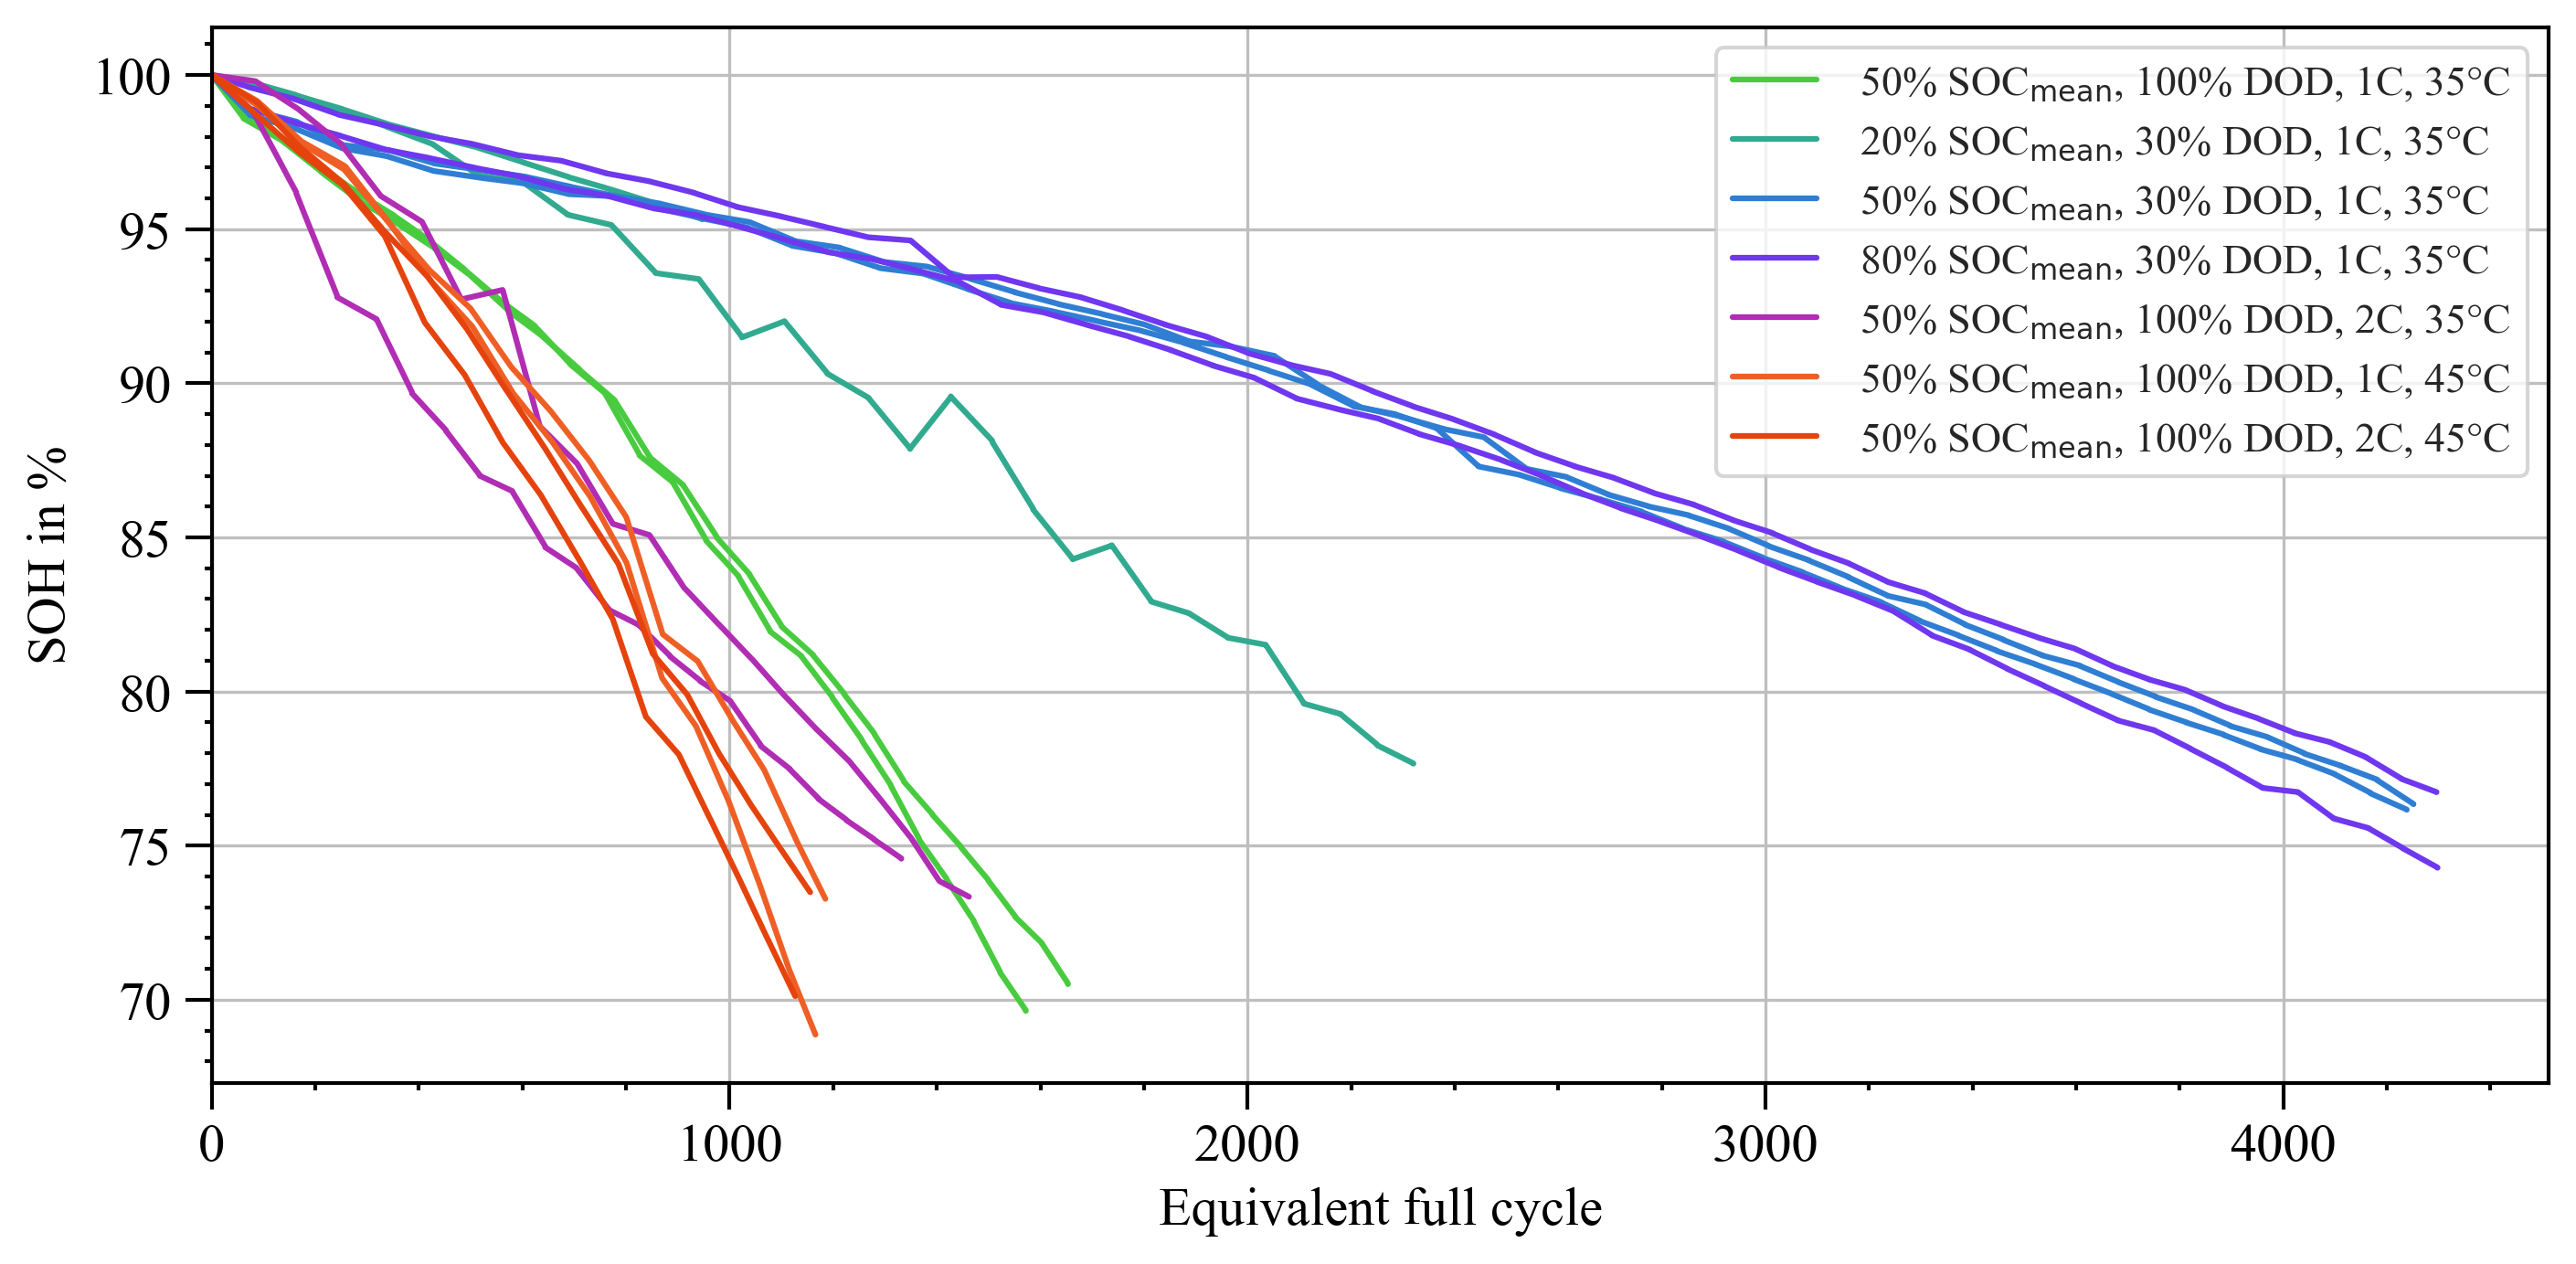
\includegraphics[width=0.8\textwidth]{Figures/SOH_n_cycle.png}
    \end{subfigure}
    \begin{subfigure}[b]{\textwidth}
        \centering
        \caption{}
        \label{fig:b}
        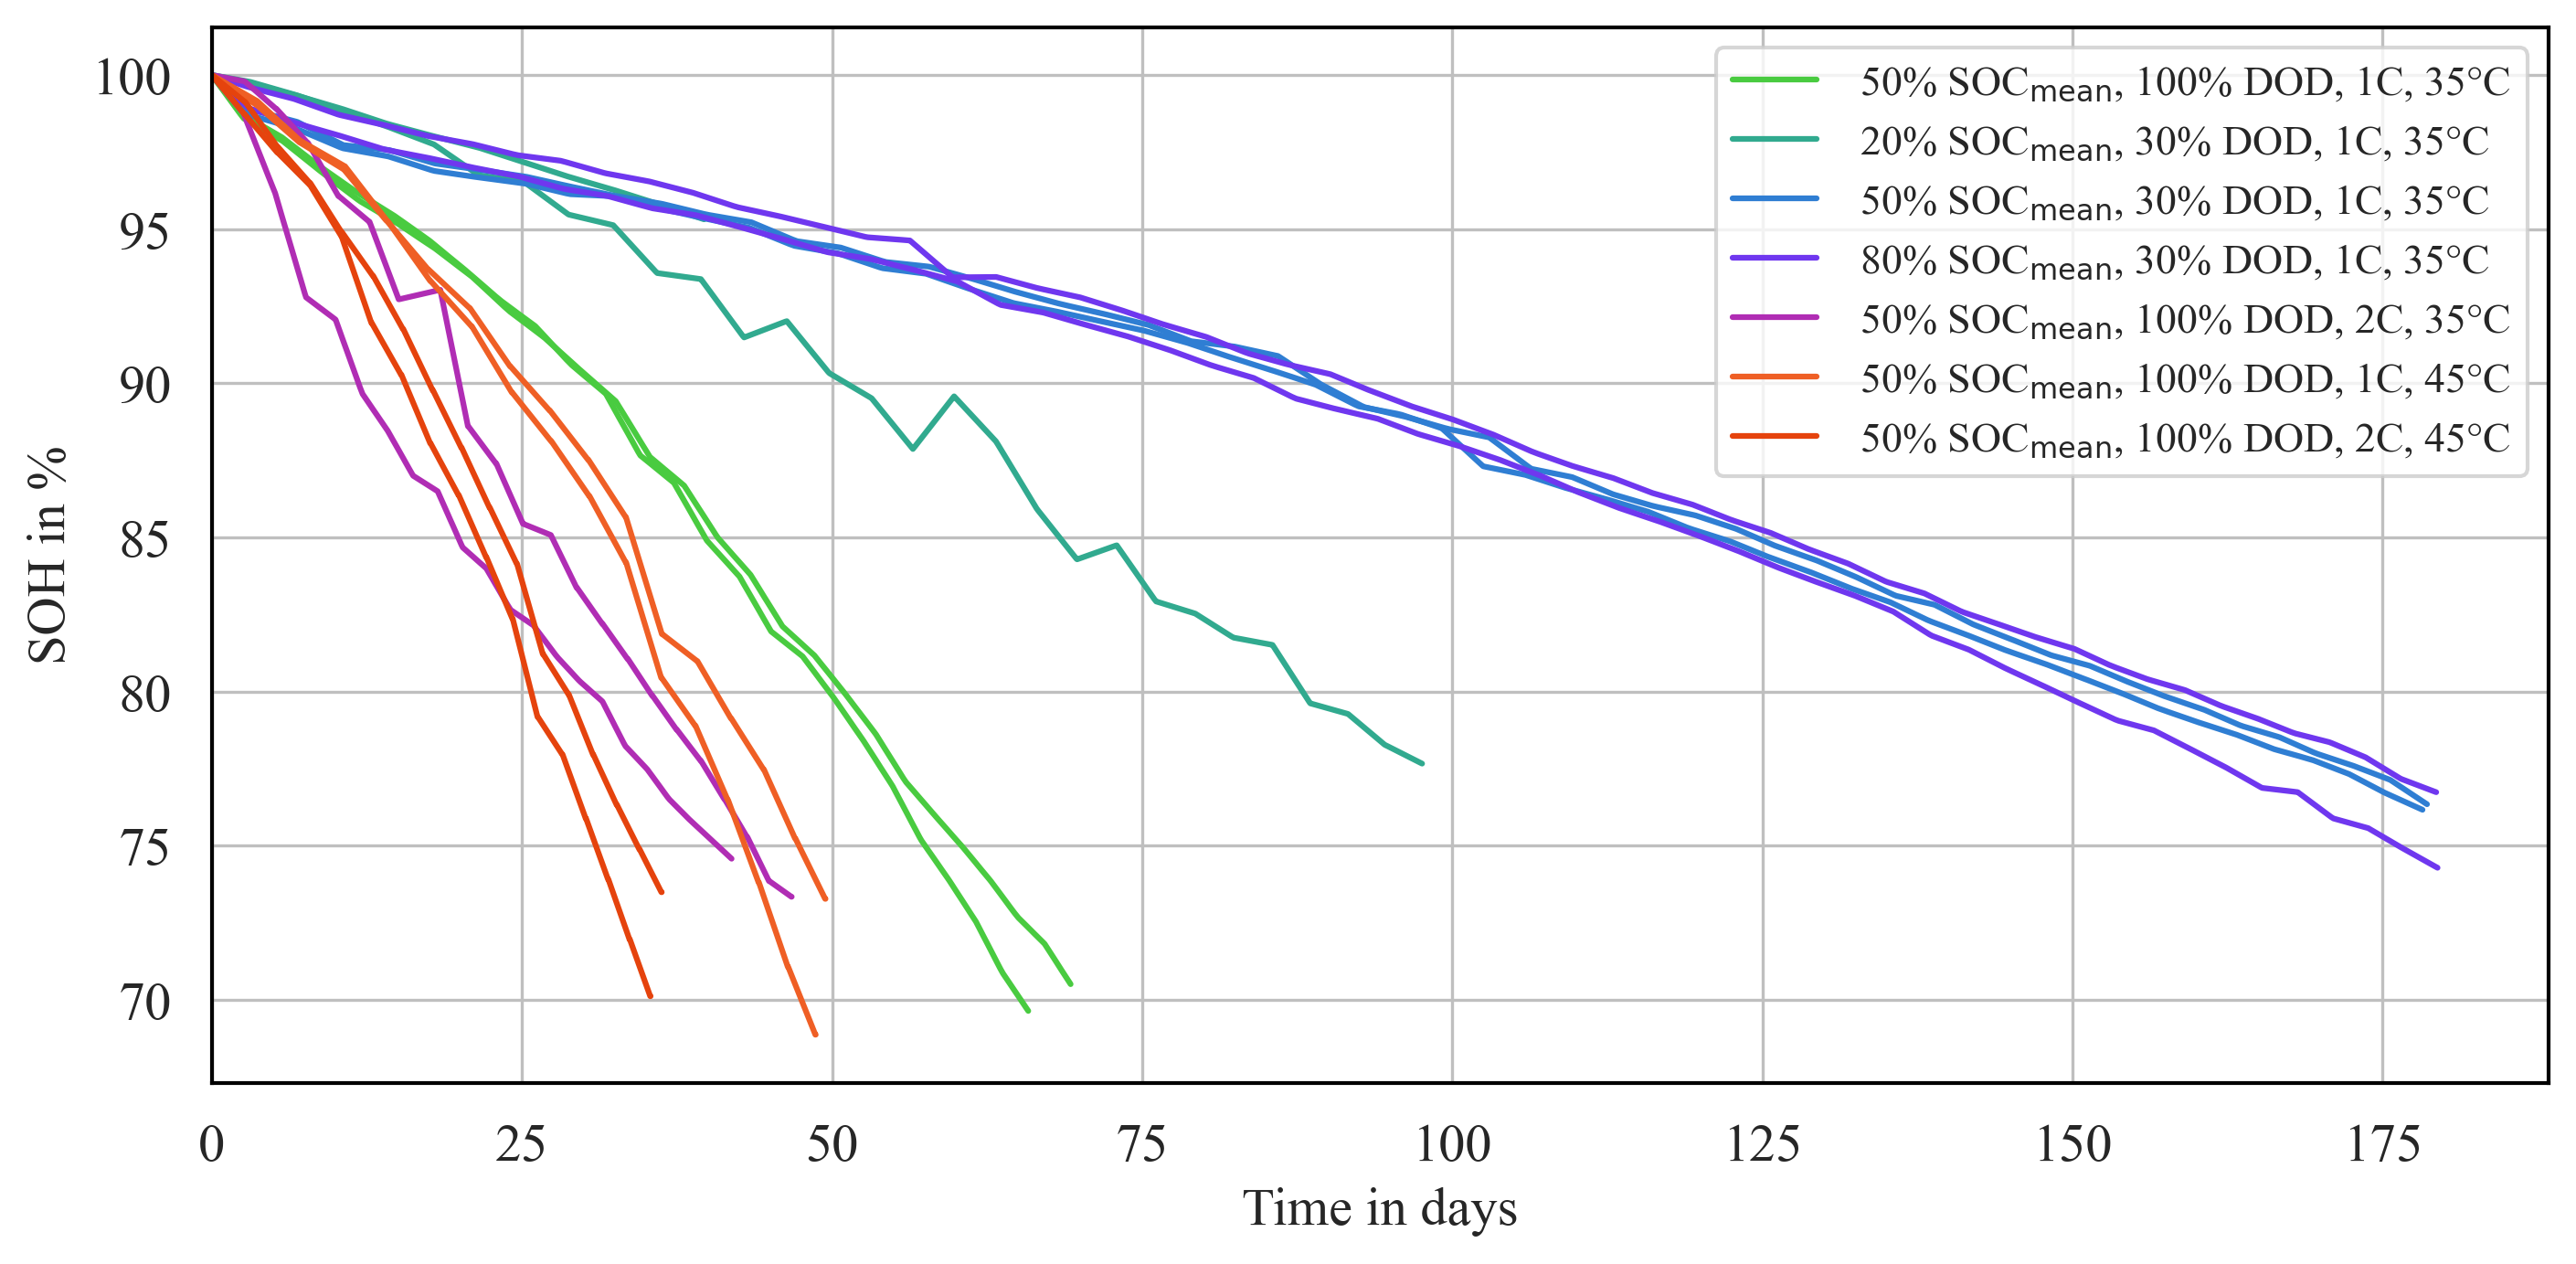
\includegraphics[width=0.8\textwidth]{Figures/SOH_t_abs.png}
    \end{subfigure}
    \caption{\hl{(\textbf{a})} Representation of the State of Health (SOH) over the equivalent full cycles for the 14 cells investigated, with each color corresponding to a specific scenario. (\textbf{b}) Temporal representation of SOH, aiding the neural network in determining the temporal change of SOH. Each scenario involves two cells under examination.}%MDPI: Figure moved after first citation, please confirm.
\label{fig:SOH}
\end{figure}

An initial analysis of the diagrams suggests that temperature significantly influences cell aging. However, the effects of other parameters and their mutual interactions are less obvious from the diagrams alone. To better understand these complex relationships, a correlation matrix was created to investigate the relationships between SOH and the various parameters. The results of this correlation analysis provide valuable insights into which parameters may be necessary for further examination and training of the neural~network.

The correlation analysis in Figure \ref{correlation_heatmap} indicated that temperature and cumulative current (both positive and negative) directly impact the SOH. In contrast, the change in voltage over time, which is also strongly dependent on temperature, has no direct influence on the SOH. However, it should be noted that a correlation analysis can only detect linear dependencies and therefore serves only as a starting point for further investigations. The neural network can identify non-linear relationships, so parameters that appear to have no direct impact on the SOH in the correlation analysis may indeed have an influence. Nevertheless, parameters directly impacting the SOH should definitely be used as inputs for the neural network.

\begin{figure}[H]
   % \centering
    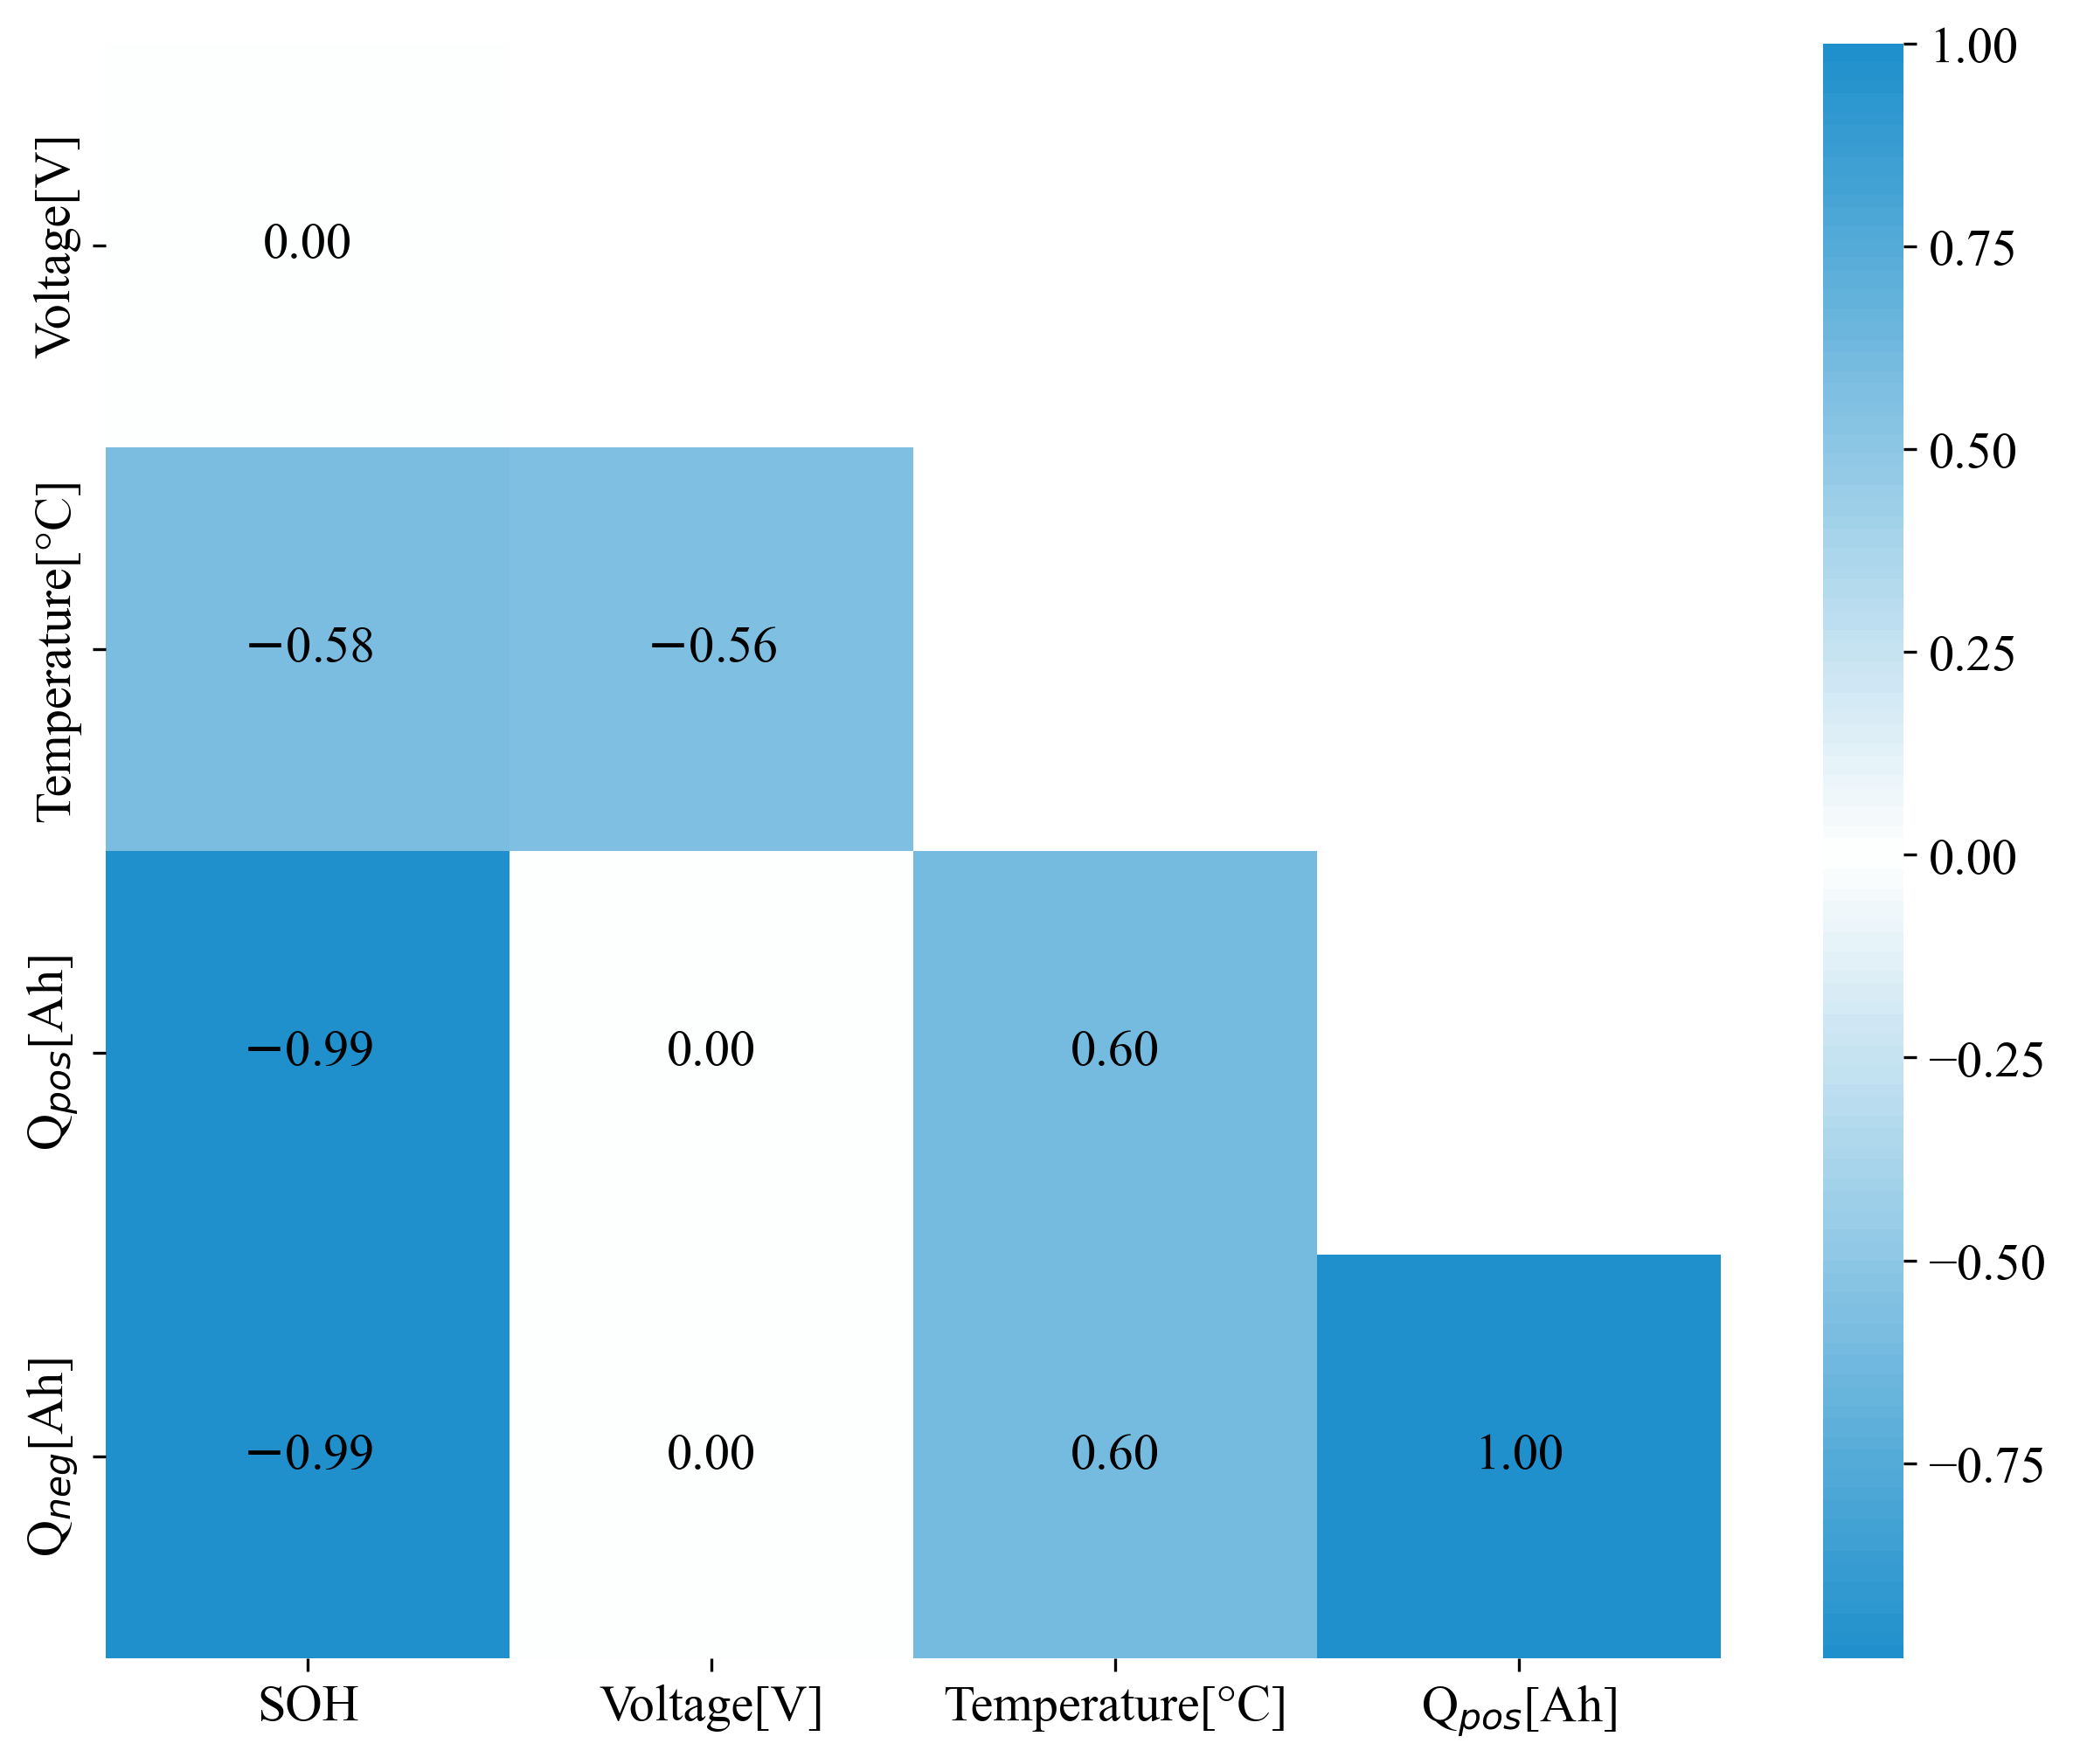
\includegraphics[width=8.5cm]{Figures/correlation_heatmap_blue_pale_dreieck.png}
    \caption{\hl{Correlation} heatmap demonstrating the relationship between various parameters such as temperature, cumulative current Q (both positive and negative), and the State of Health (SOH). A value close to +1 or $-$1 indicates high correlation, while a value close to 0 indicates no correlation. Linear dependencies are highlighted, providing a foundation for further investigations. %MDPI: Please change the hyphen (-) into a minus sign ($-$, "U+2212") in the image. e.g., "-0.58" should be "$-$0.58".
    \label{correlation_heatmap}}
\end{figure}





\subsection{Formation of the Lag Sequence}

The structure of a sample utilizes a lag sequence based on a cell measurement. This sequence employs the features of voltage, temperature, and cumulative current as inputs from the data set while adopting the SOH as the label, as shown in Figure \ref{fig:LagSequence}. Including past input values aids in enhancing prediction accuracy, with sliding windows defining the temporal duration of the lag sequence.

\begin{figure}[H]
%\centering
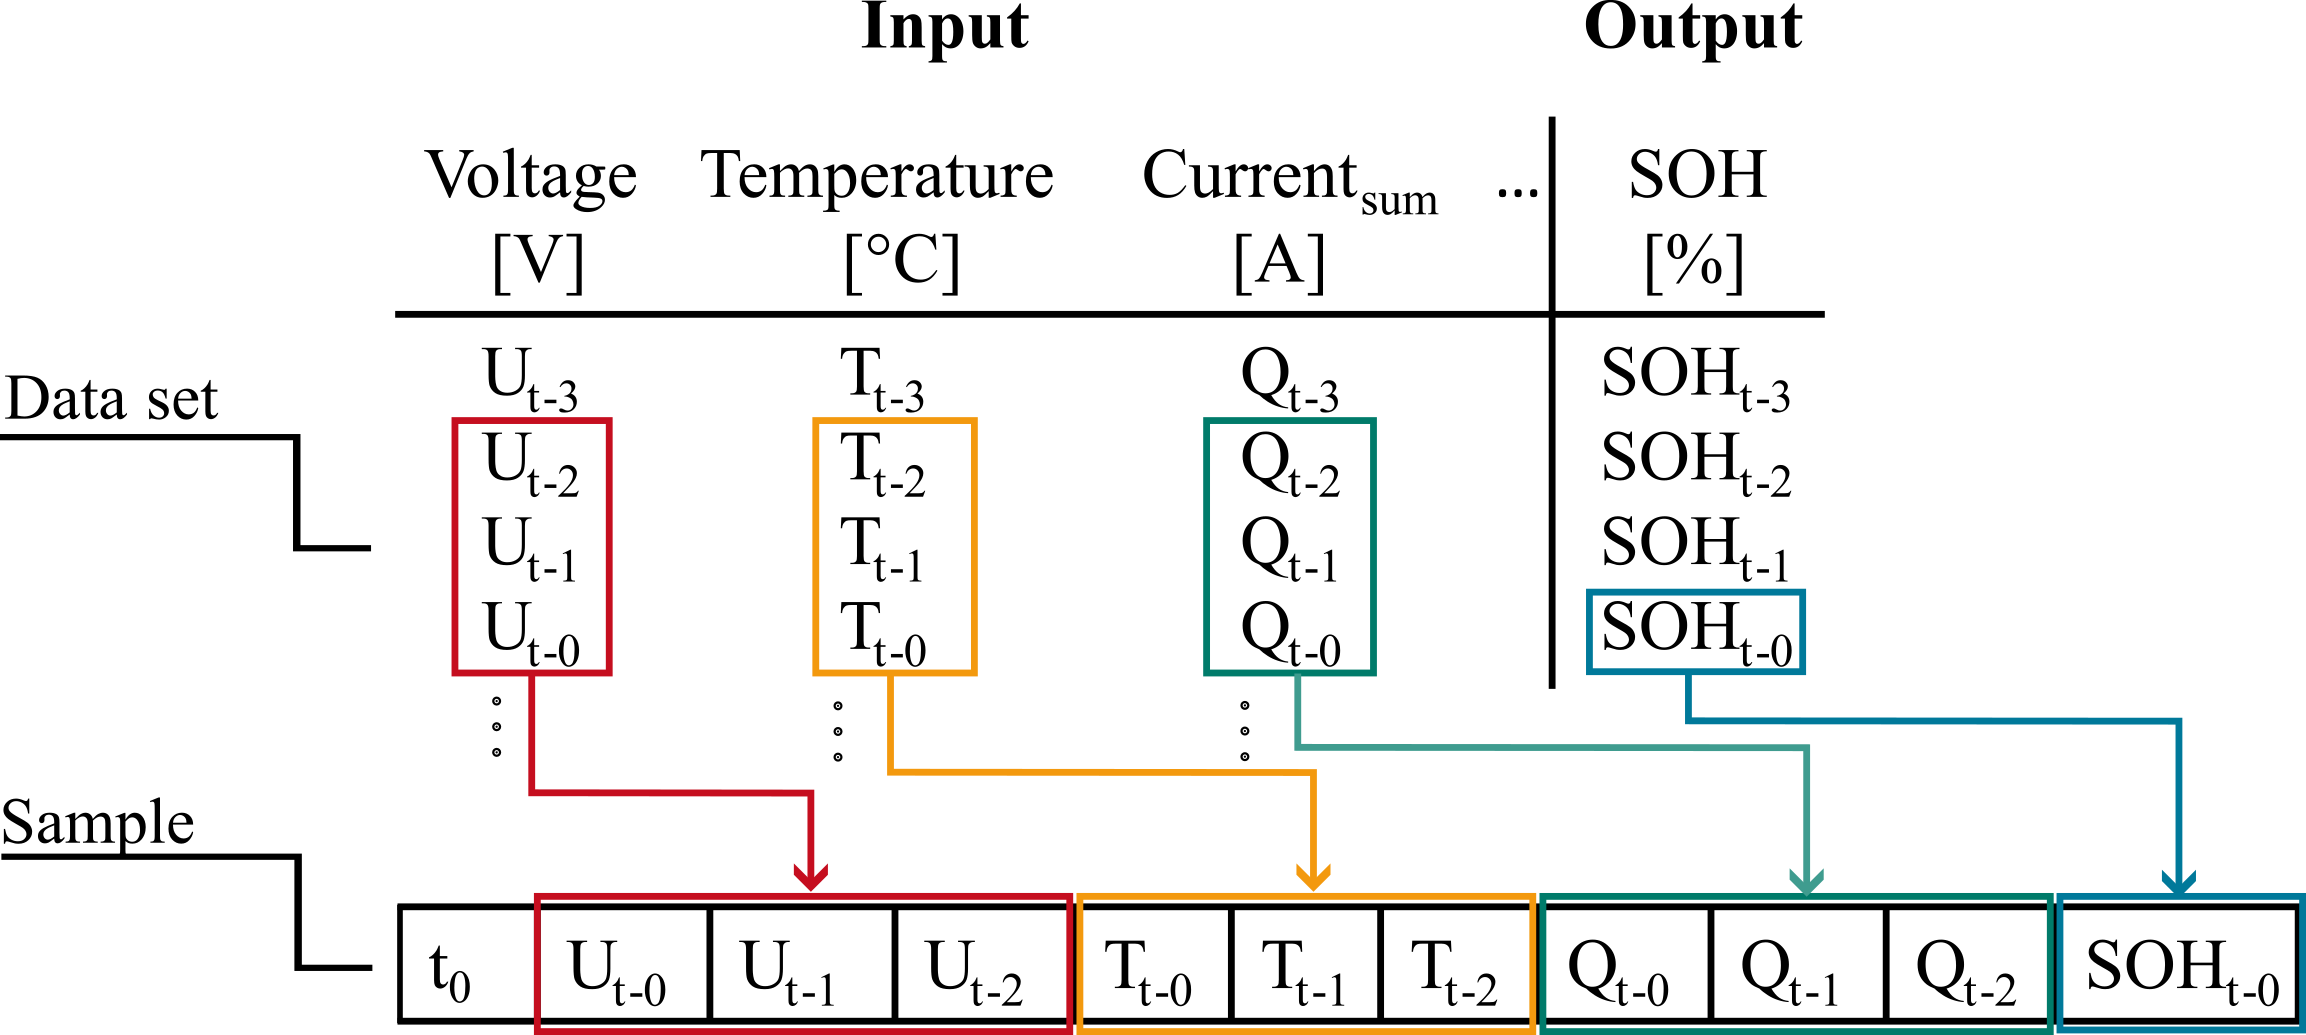
\includegraphics[width=10.5cm]{Figures/NN_MLP_Tabelle.png}
\caption{Illustration of forming a lag sequence sample for the neural network based on cell data. The table demonstrates the transformation of raw input parameters, such as voltage, temperature, and cumulative current, into a structured lag sequence. Each sequence's output, or label, is the State of Health (SOH). The dataset depiction shows the conversion of real-time cell data into a learning sample for the neural network, highlighting the transformation process that facilitates efficient model training.\label{fig:LagSequence}}
\end{figure}

The time resolution is initially set at 30 min, a choice that depends on factors such as usage patterns, discharge and charge times, and profiles, such as high currents in a short time, which can influence the selection. Subsequently, the number of sequences is determined, resulting in the overall duration or history of the data used for network training. In this case, choosing a number of 12 sequences represents the past 6 h of data ($12 \cdot$ 30 \hl{min}). %MDPI: We removed the italics. Please confirm this revision.


The optimal configuration between the number of sequences and time resolution is further refined during hyperparameter optimization. If pulses fall within this time, they are reflected in the average value of the input parameters. When designing the sequences, the sampling theorem \cite{PuenteLeon.2015} must be considered to ensure that the network can recognize the periodic charging and discharging cycles. The spacing between individual data points determines the temporal resolution.

Noise is not a consideration for the estimation process in this study, as the proposed feature engineering method involves the resampling of the measured data. This resampling effectively works as a low-pass filter, which greatly dampens noise fluctuations. By considering the sampling theorem \cite{PuenteLeon.2015} and ensuring the appropriate spacing between individual data points, the method allows for the recognition of periodic charging and discharging cycles while minimizing noise components. This lets us assume that noise components in the final estimation are minimal in relation to the mean of the prediction. %v3.0%

The SOH for the current point in time is determined based on various inputs. Forming lag sequences makes it possible to utilize the entire dataset from all cells for training. Instead of supplying the model with the data from an entire cell for training, only individual sequences of cumulative current, voltage, temperature and SOH are used.

The lag sequences render the data presented to the network independent of any specific cell. This allows random training with the sequences, preventing the network from learning specific behaviors of individual cells.

\subsection{Training, Validation, and Test Splits}

The assessment and calibration of a neural network model's effectiveness and adaptability require the implementation of training, validation and test splits, as observed in Figure~\ref{process}. Training data modify the model's weights and biases, aligning them with the known input and output pairs. On the other hand, the validation set tests the model's handling of unseen data during training. This is crucial for identifying potential issues, such as overfitting---a scenario where the model becomes too attuned to the training data, performing sub-optimally on fresh data. The validation data assists in monitoring the model's performance, allowing adjustments such as hyperparameter tweaking to better its adaptability.

The test set serves as an independent evaluation pool that the model has not encountered during training. It objectively estimates the model's effectiveness on new, unseen data. It lets us evaluate the model's adaptability to various scenarios and provides a reliable performance measure. The model's performance evaluation becomes more robust by using distinct training, validation, and test splits. This method assists in pinpointing potential problems before the model's deployment in real-world scenarios. Initially, 20\% of the training sequences are set aside for validation, but the optimization process could consider using fewer data points for validation while maintaining accurate approximation.

Model training happens only with a portion of the total dataset, with 4 out of 14 cells retained for the final accuracy assessment. The remaining data are split further into training and validation sets. The validation set is used during training to test the model's current state on unseen data, which assists in checking whether the model is overfitting and incapable of generalizing beyond the training data. Overfitting occurs when the model becomes overly accustomed to the training data, leading to lower prediction errors on the training set but higher errors on unseen data. Once the model is fully trained with the training and validation data, it is then tested using the test data (the remaining three cells) to evaluate its final performance with unfamiliar data. 


\subsection{Data Scaling}

Data optimization also includes scaling the features to values between 0 and 1. Scaling data aids in improving the neural network's convergence during training and ensures that all features possess a comparable range of values, thus enhancing the efficiency of the learning process. Non-uniform scales can result in certain features dominating and others being neglected, leading to subpar model performance \cite{Salimans.2016}.

By reducing the influence of large values that could potentially cause numerical issues, scaling supports the model's numerical stability. Uniform scaling facilitates the comparison and interpretation of weights and bias values within the layers of the neural network. This is particularly important when different input variables have varying units or scales, to ensure proper comparability.

Both the training dataset and the validation and test datasets must be scaled to guarantee consistent results and comparability across sets. This ensures that the weights of the neural network do not favor large absolute values and neglect small absolute values. For instance, cell voltages range from 2.75 V to 4.2 V, while cumulative currents rise up to several thousands Ah. This discrepancy can significantly influence the weights, thus underlining the necessity of data scaling.


%%%%%%%%%%%%%%%%%%%%%%%%%%%%%%%%%%%%%%%%%%
\section{Multilayer Perceptron Neural Network Model Structure}

The work employs a Multilayer Perceptron (MLP) neural network model, owing to its aptitude for handling structured and non-spatial data dependencies. This choice was made after considering other network architectures, such as Convolutional Neural Networks (CNNs) and Long Short-Term Memory (LSTM) networks.

CNNs, while highly effective in tasks involving image data or where spatial dependencies must be captured, do not present substantial advantages when processing structured data that lacks inherent spatial relationships. In contrast, LSTMs are designed for sequential or time-series data and can learn long-term dependencies effectively. Nevertheless, they may be resource-intensive and computationally demanding, making them less suitable for applications where fast training and prediction times are crucial, or resources are~limited~\cite{Li.20182016}.

MLPs, with their feedforward architecture, have proven to be effective and efficient in processing structured data. By creating lag sequences, temporal patterns within each sequence can be captured, offering a practical solution even for time-dependent data. Furthermore, MLPs are less prone to training difficulties and are easier to optimize due to fewer hyperparameters compared to LSTMs~\cite{Weytjens.2021}.

The MLP model (see Figure \ref{NN_MLP}) used in this work comprises at least three layers: an input layer, one or more hidden layers, and an output layer. The number of nodes in the input layer equals the number of input features in a sample.

In the initial setup, each hidden layer consists of eight nodes, each fully connected to all nodes in the previous layer. However, the exact architecture in terms of nodes per layer may vary based on the specific use case and data situation and should be determined through hyperparameter tuning.

Each neuron, except those in the input layer, is equipped with a Rectified Linear Unit (ReLU) activation function, which transforms the weighted inputs into an output. During the training process, the weights connecting the neurons between layers are adjusted to enhance the model's predictive performance.

The output layer comprises a single node, representing the estimated value of the target variable: the cell's State of Health (SOH). The model's objective is to minimize the error between the predicted and true SOH values; it is evaluated using the Mean Squared Error loss function that is commonly used for regression tasks. %Please verify.

\begin{figure}[H]
%\centering
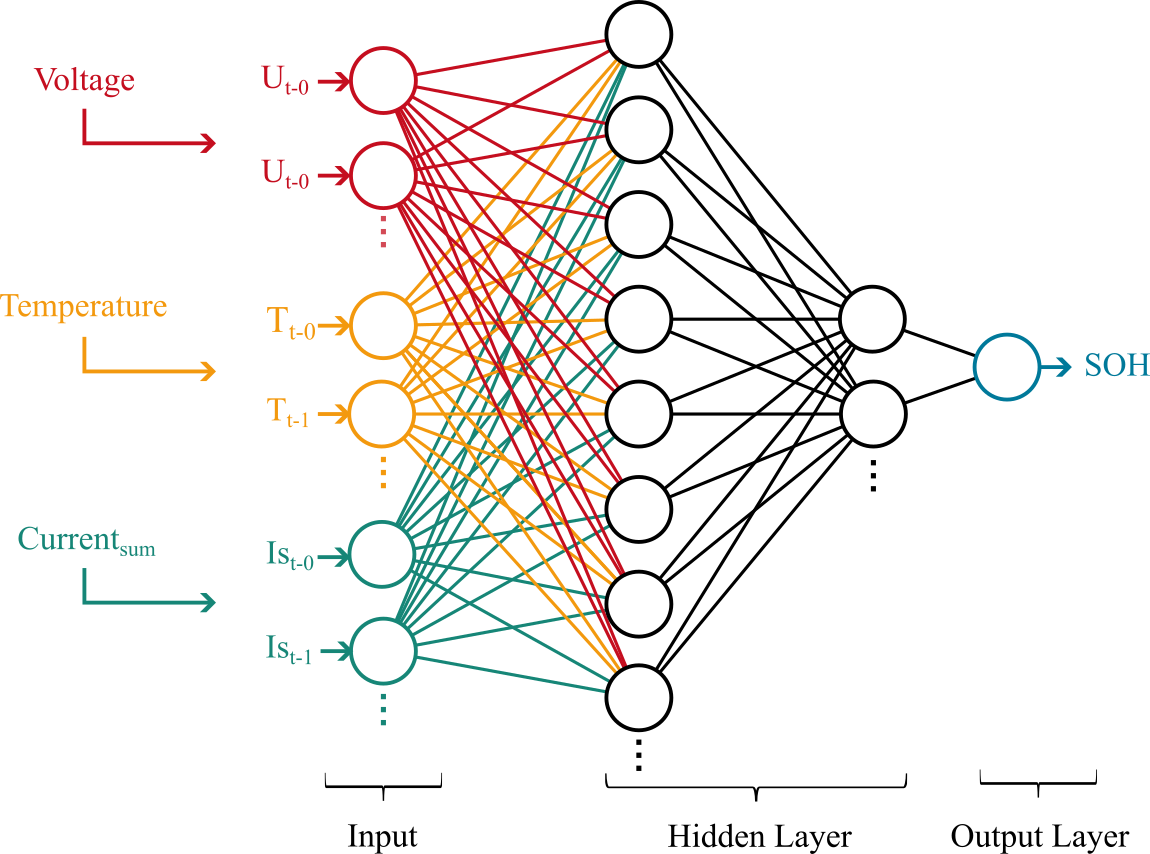
\includegraphics[width=10.5cm]{Figures/NN_MLP.png}
\caption{\hl{Illustration} %MDPI: Please cite the figure in the text and ensure the first citation of each figure appears in numerical order.
 of the Multilayer Perceptron (MLP) neural network model used for predicting the State of Health (SOH) of a cell. The network takes as inputs voltage, temperature and cumulative current. The number of input nodes can vary depending on the number of sequences. Each input node is connected to every node in the hidden layers, which is characteristic of an MLP structure. The model produces the SOH estimate from a single output node. The figure highlights the interconnected nature of the network, demonstrating the flow of information from inputs through hidden layers to the final output. \label{NN_MLP}}
\end{figure}

%%%%%%%%%%%%%%%%%%%%%%%%%%%%%%%%%%%%%%%%%%
\section{Evaluation Methods}

The performance of the neural network, employed to estimate the State of Health (SOH), was evaluated using the Mean Squared Error (\hl{MSE}) during training and validation. The \hl{MSE} is defined as: %MDPI: Variables should be in the same format in formulas and paragraphs. Please confirm whether italics are required. The following highlights are the same.
\begin{linenomath}
\begin{equation}
MSE = \frac{1}{n} \sum_{i=1}^{n}(y_i - \hat{y}_i)^2
\end{equation}
\end{linenomath}
where $n$ is the number of samples in the dataset, $y_i$ is the actual value of the $i$-th sample, and $\hat{y}_i$ is the predicted value of the $i$-th sample.

The h was used as a metric to assess the accuracy of the MLP's predictions against the actual SOH values. During the training process, the objective was to minimize the MSE to achieve better data fitting.

Several experiments were conducted by modifying parameters such as the number of nodes, sequence resolution, and network depth. In each case, the network's performance was measured using the \hl{MSE}.

The changes in the number of nodes and sequence resolution were tested, and their impacts on the model's prediction accuracy were assessed using the MSE. The network's depth was also varied, and the resulting MSEs were used to gauge the performance of the MLP with different architectural configurations.

During the validation phase, the MSE was used to evaluate the performance of the trained network on new data using a separate validation dataset.

After training and validation, the model was tested with an independent test dataset. The performance was evaluated using the MSE and the Mean Absolute Error (\hl{MAE}). The MAE is defined as:

\begin{linenomath}
\begin{equation}
MAE = \frac{1}{n} \sum_{i=1}^{n} |y_i - \hat{y}_i|
\end{equation}
\end{linenomath}

\hl{MAE} measures the error in the original units of the target variable, making it easier to interpret than the MSE. This can be particularly useful when the neural network's predictions need to be interpreted directly.

Both the MSE and the MAE were used to evaluate the accuracy and quality of the predictions made by the neural network, ensuring that it performs well on unknown data.

The final test with the independent dataset was used to evaluate the model's actual performance, with the MSE and MAE serving as the evaluation metrics.

\section{Configuration and Hyperparameter Tuning of the Neural Network}

This section discusses the initial choice of a Multilayer Perceptron (MLP) with specified initial conditions and subsequent fine-tuning with hyperparameter tuning. An initial explanation will focus on the typical impact of individual parameters, such as the number of nodes, network depth and other parameters.

\textbf{\hl{Hyperparameter tuning:} %MDPI: Please confirm if the bold is necessary. The following highlights are the same.
} The hyperparameter tuning process automatically adjusts the parameters. The parameters specifically crucial in this work were those of the lag sequence: the number of sequences and time resolution. These will be examined in greater detail and will be closely scrutinized in the evaluation of the results. The hyperparameter tuning process also includes the Hyperband approach, which optimizes hyperparameters through intelligent resource budgeting. It conducts multiple ``bands'' of experiments, each using a specific number of epochs for training. Within a band, many hyperparameter configurations are tested, but only the most promising receive additional resources. By quickly discarding less promising options, Hyperband allows for a more efficient search in the hyperparameter space, often resulting in faster and better results compared to traditional methods \cite{Li.20182016}. %v.3.0

\textbf{\hl{Nodes:}} The number of nodes in the network significantly impacts its performance. By increasing the number of nodes in the network, the network's capacity can be enhanced, enabling it to capture more complex patterns and relationships.

\textbf{\hl{Network Depth:}} Greater network depth allows the network to learn hierarchical features and abstract relationships in the data. This enhanced capacity improves its ability to handle more complex problems. Additional hidden layers are added based on this model. Nodes used in the later layers are compelled to learn the data's most essential and discriminating features, while less relevant information is attenuated or ignored. This process helps prevent overfitting because the model is less likely to memorize specific examples from the training dataset and instead recognizes more general patterns. Therefore, the model's generalization ability is improved, and it is better equipped to classify unknown data accurately. The MLP used as the starting point had a single hidden layer and eight nodes.

\textbf{\hl{Additional Parameters}:} Additional factors that influence the network's performance include batch size, regularization, optimizer type, and activation function.

The choice of batch size can impact the stability and efficiency of the training process. Larger batch size can lead to faster training but may also result in lower generalization ability. Conversely, a smaller batch size can improve generalization but may require more computational resources and longer training times.

The model was tested with 15,000 sequences with various distributions of batch size and epoch count. All models achieved similar absolute convergence, but a larger batch size decreased overfitting.

Kernel regularization was also examined to determine whether it could improve the model. However, regularization only increased the absolute minimum value, with no other improvements observed.

The impact of different optimizers was also tested. ADAM outperformed RMSProp, Adadelta, and Adagrad. ADAM combines a dynamic adjustment of the learning rate with momentum, while the other optimizers only cover aspects of these features.

Regarding activation functions, ReLu generated the most minor loss compared to other functions such as Sigmoid, Tanh, or Softmax. The results of the network architecture can be seen in Table \ref{tab:neural_network_config}.


\begin{table}[H]
\caption{\hl{A} configuration of the neural network used in the experiment, indicating the number of nodes and the respective activation functions in each layer.}%MDPI: Please cite the table in the text and ensure the first citation of each figure appears in numerical order.
\label{tab:neural_network_config}
\newcolumntype{C}{>{\centering\arraybackslash}X}
\begin{tabularx}{\textwidth}{CCC}
\toprule
\textbf{Layer} & \textbf{Nodes} & \textbf{Activation Function} \\
\midrule
0 & 128 & ReLU \\
1 & 256 & ReLU \\
2 & 256 & ReLU \\
3 & 256 & ReLU \\
4 & 128 & ReLU \\
5 & 512 & ReLU \\
6 & 128 & ReLU \\
7 & 256 & ReLU \\
8 & 256 & ReLU \\
9 & 1 & Linear \\
\bottomrule
\end{tabularx}
\end{table}

The following section dedicated to evaluating results will provide a more detailed analysis of the effect of the number of sequences (quantity of lag sequences or the duration of a lag sequence) and time resolution.

\section{Results and Performance Evaluation}
The number of sequences and time resolution are additional parameters that warrant detailed examination in this study. The evaluation of these parameters aims to ascertain the influence of the number of sequences and the precision of the time resolution on the final results.

As detailed in \hl{Section} \ref{sec3}, the lag sequence depends on the usage as well as discharge and charge times. If the sampling of data points, or the time resolution, is too large, vital information may be lost. On the other hand, the evaluation revealed that a time resolution that is too small can also be disadvantageous. This is primarily due to the Vanishing Gradient Problem, where information can be lost during backpropagation in training deep neural networks, making it challenging for the model to learn and tune its parameters effectively.
%MDPI: Chapter changed to Section, please confirm.

In \highlighting{Figure \ref{MAE_matrix}},  %MDPI: The first citation of each figure should appear in numerical order. Please add the mention of Figure 5 before this.
three cells aged under different conditions are taken as examples. For the evaluation, four different time resolutions were selected: 1 min, 10 min, 30 min, and 60 min. The evaluation indicates an optimal range of 10 to 30 min for the time resolution. Given that discharge times vary due to differing discharge currents of 1C and 2C at DODs ranging from 30\% to 100\%, the cells are discharged and charged in intervals of approximately 20 min to 1 h. Consequently, different cells and scenarios yield different optimal time resolutions. The intention is to highlight the importance of matching the time resolution to the charge/discharge cycle duration to prevent the loss of critical information.

\begin{figure}[H]
\begin{adjustwidth}{-\extralength}{0cm}
\centering
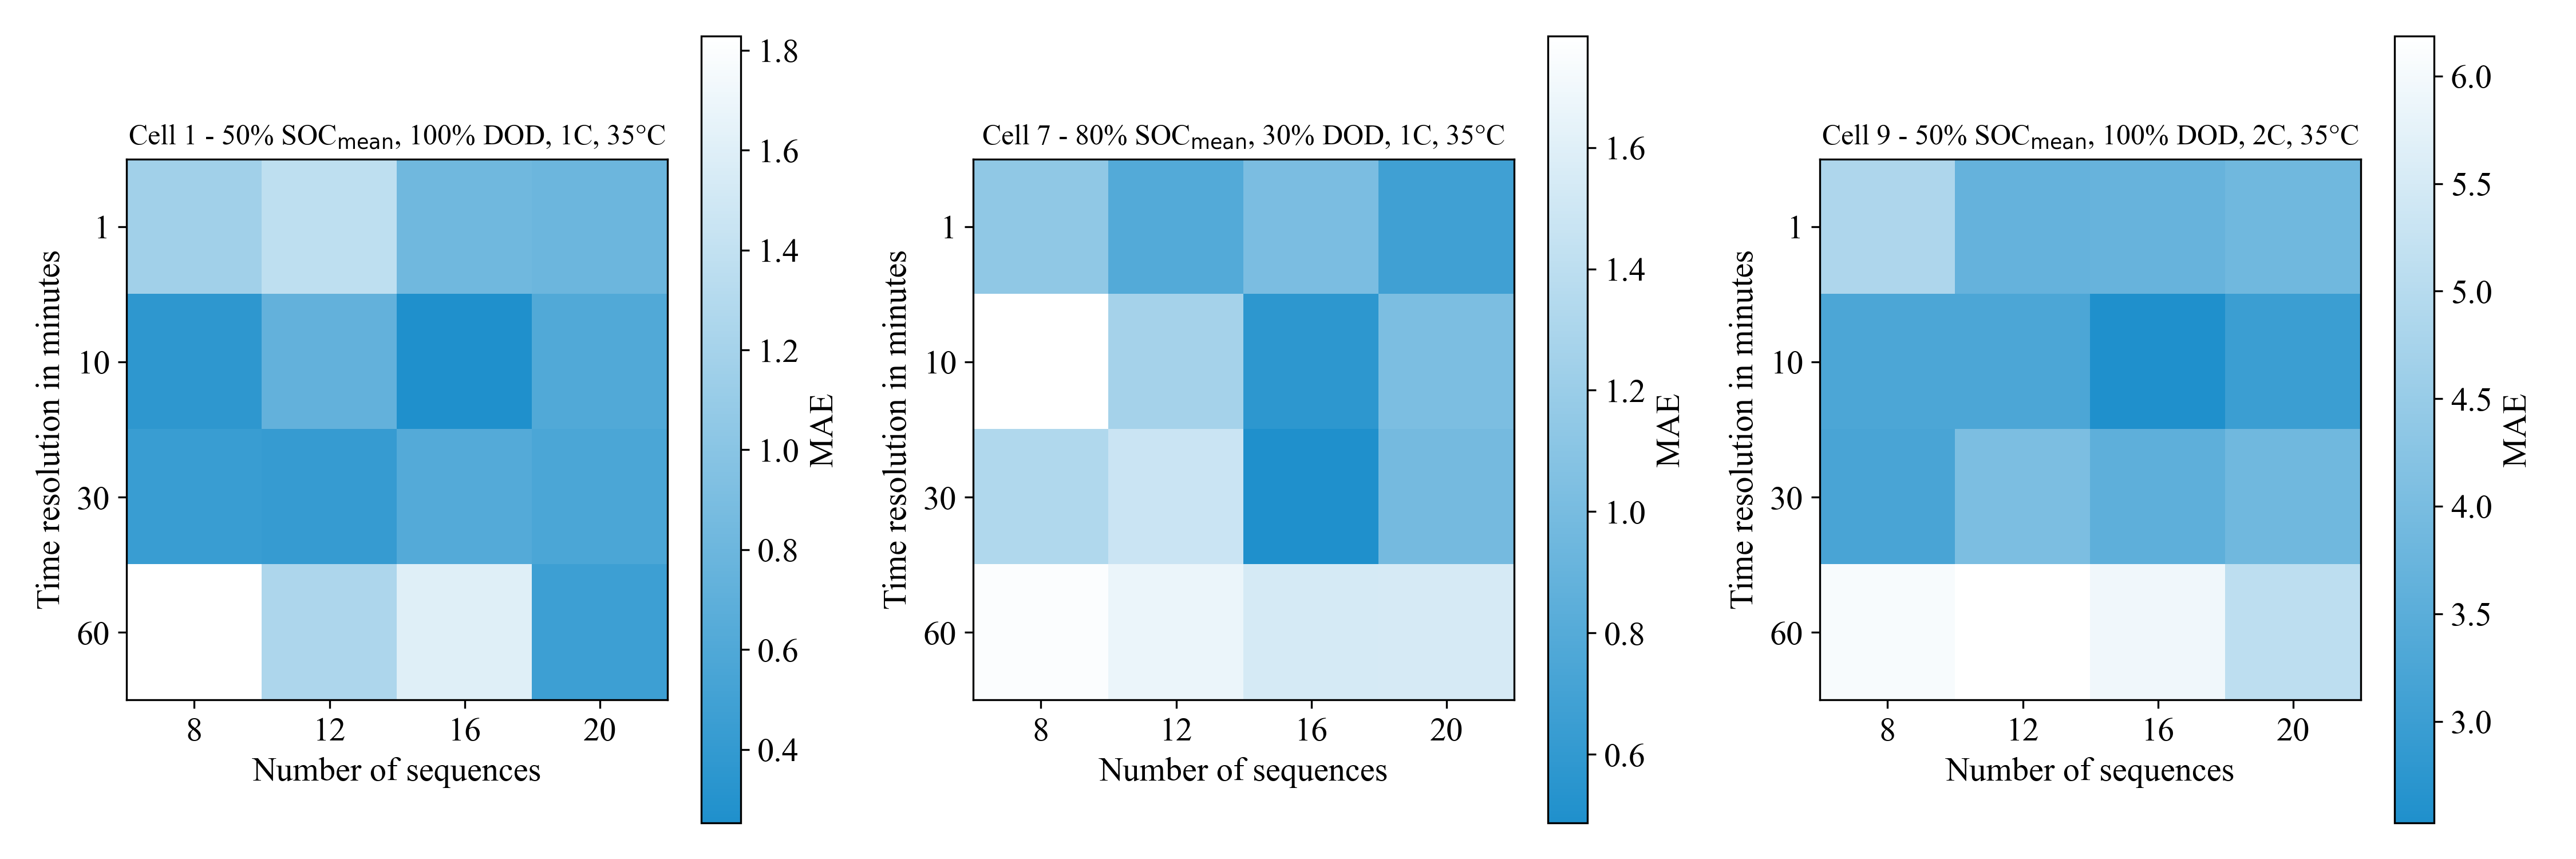
\includegraphics[width=16.5cm]{Figures/MAE_matrix.png}
\end{adjustwidth}
\caption{Matrix of MAE errors showing the correlation between number of sequences and time resolution for three test cells. The colors represent the magnitude of the error, with an optimal range of 10 to 30 min for time resolution.\label{MAE_matrix}}
\end{figure} 

The impact of the number of sequences, which refers to the total amount of historical data used for the prediction, is another critical consideration. The sequence length is determined by the multiplication of the number of sequences and the time resolution. Greater sequence lengths mean more historical data are available, but if the sequence is excessively long, overfitting can occur. Therefore, it is vital to analyze the effect of sequence length, specifically the number of sequences on prediction accuracy, as measured by the MSE and MAE. %Please verify.


For numbers of sequences set to 8, 12, 16, and 20, the trend indicates that the error tends to decrease as the number of sequences increases. However, it is essential to find an optimal point, which depends on the setting of the time resolution. The experiments demonstrated that extending the number of sequences beyond 20 was not advantageous due to an excessively long data history.

The MAE error matrix reveals that the error is smallest with a sequence length determined by 16 sequences and a time resolution of 10 min for all exemplary test cells. This would correspond to a historical data length of 160 minutes.

Mean Squared Error (MSE) and Mean Absolute Error (MAE) are used to validate the prediction accuracy of the MLP. Figure \ref{SOH_SOH_pred} compares the predicted SOH and the actual measured SOH over time. The diagrams for Cell 7 and Cell 1 represent the typical aging process of an NMC cell, which is most frequently observed in evaluations. In both cases, the SOH is very well estimated by the neural network.

\begin{figure}[H]
\begin{adjustwidth}{-\extralength}{0cm}
\centering
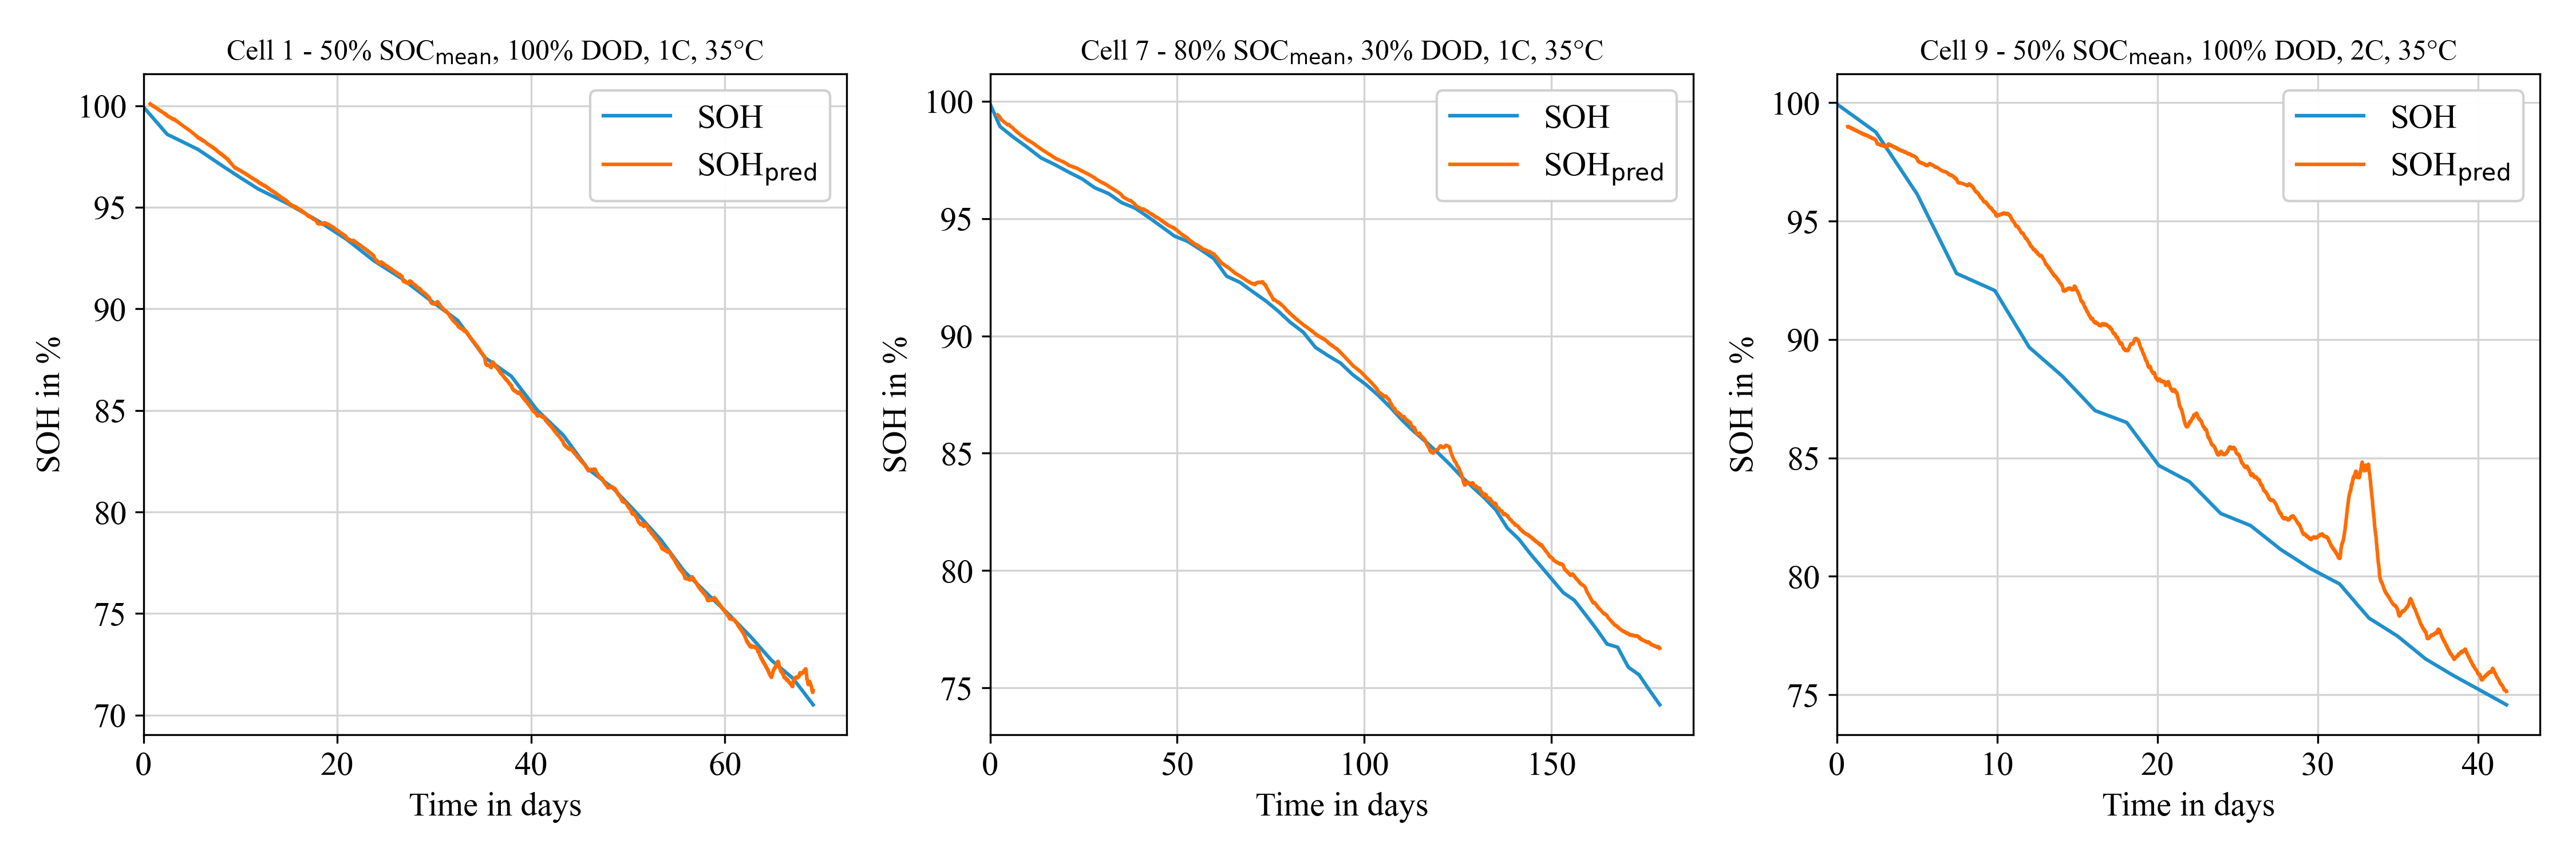
\includegraphics[width=16.5cm]{Figures/SOH_SOH_pred.png}
\end{adjustwidth}
\caption{\hl{Comparison} of predicted and actual State of Health (SOH) over time for three test cells. Cells 7 and 1 show typical aging progression, whereas Cell 9 exhibits an atypical U-shaped curve. A post-rolling filter was employed to reduce data noise to enhance results and smooth the data. \label{SOH_SOH_pred}}
\end{figure}
%MDPI: Figure moved after first citation, please confirm.


However, Cell 9 presents a different case. This cell was specifically selected for an evaluation to demonstrate how the MLP handles atypical measurements. Cell 9 has a rather atypical progression, featuring a U-shaped curve, which deviates significantly from the other cells. The SOH of this cell is estimated with a more significant error. This selection was intentional to illustrate the challenges and capabilities of the MLP in dealing with unconventional SOH trajectories. The inclusion of Cell 9 in the evaluation explains the larger error observed in the results, showcasing the network's response to non-standard behavior. %v.3.0

The evaluations in Figure \ref{SOH_vs_SOH} yielded the best SOH estimates with MSE values of 0.410 and 0.118 and MAE values of 0.487 and 0.253. These values measure the average square and absolute deviation between the predicted and actual SOH values.

\begin{figure}[H]
\begin{adjustwidth}{-\extralength}{0cm}
\centering
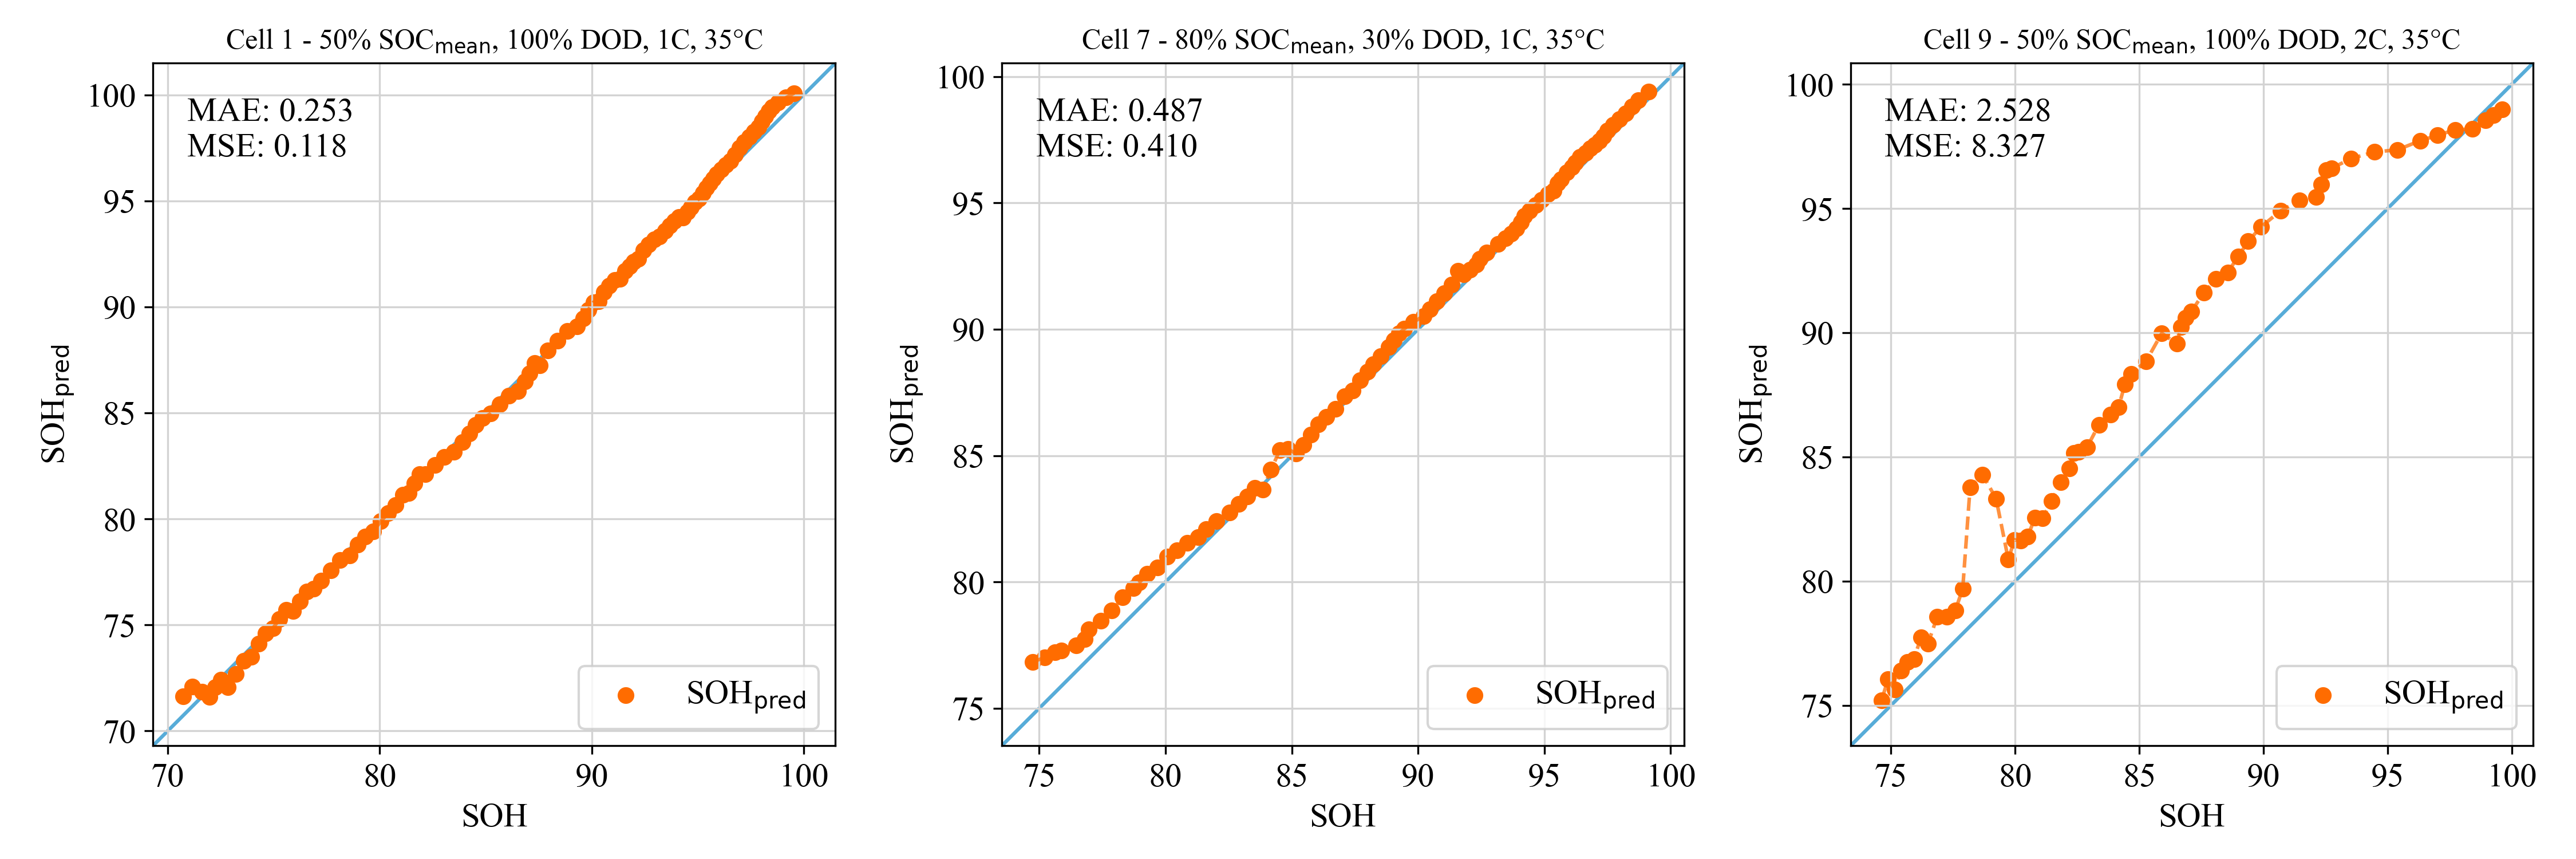
\includegraphics[width=16.5cm]{Figures/SOH_vs_SOH_pred.png}
\end{adjustwidth}
\caption{\hl{Plot} of predicted SOH values against actual SOH for three test cells. Cells 7 and 1 show small dispersion and low absolute error, indicating accurate prediction, while Cell 9 displays high deviation in both MSE and MAE.\label{SOH_vs_SOH}}
\end{figure}
%MDPI: Figure moved after first citation, please confirm.

A lower MSE value indicates that the MLP's predictions are, on average, relatively close to the actual SOH values and have less dispersion. Conversely, a higher MSE suggests a greater average squared deviation of the predictions from the actual values, indicating a higher variance in the predictions. The MSE is sensitive to larger deviations and outliers, as it uses the squared deviation.

A lower MAE value indicates that the MLP's predictions are, on average, relatively close to the actual SOH values. A higher MAE suggests a greater average absolute deviation of the predictions from the actual values. The MAE allows for easy interpretation, as it measures the deviation in the original units of the target variable, in this case, the SOH values in percentage.

In the context of the test evaluation, a small MSE represents a small dispersion of results, while a large MSE represents a large dispersion of results. It is important to note that outliers can heavily influence the MSE, as larger deviations are quadratically weighted more heavily.

To visually represent the deviation of the values, the predicted SOH values were plotted against the actual SOH. If the predicted SOH matches the actual SOH, it lies exactly on the plotted line in the diagram.

In the first two diagrams for Cell 7 and Cell 1, there is very little dispersion, and the absolute error is very small, corresponding to a good prediction. Cell 9, on the other hand, shows a high deviation in both MSE and MAE.
    


On average, a value of 1.10 for the MAE and 2.95 for the MSE was obtained. These metrics provide a valuable measure of the model's accuracy and reliability, enabling an understanding of how well the model is performing and where improvements can be made.

In the tests in which cells 3 and 4 were removed from the training set, i.e., those which were terminated prematurely and produced relatively unusable results, an improvement in the final result was noted. In the previous trial with the same test cells, the MAE was reported to be 1.07, with the MSE averaging 2.52. The excision of the corrupt cells contributed to a marginal improvement in the results, although this intervention led to an increasingly unstable pattern in cell 9, with the SOH showing significant fluctuations.

\textls[-25]{When choosing the appropriate parameters---time resolution and number of sequences---it might be appropriate to also consider the general usability of the SOH$_{pred}$. A suitable evaluation metric should be sought for this. The experiment with corrupt data removal underlines the strong dependence of this method, as with all machine learning approaches, on the underlying data. The availability of a larger data set correlates with the precision of the achievable results.}

Hence, with the presented method, it is challenging to provide a precise recommendation for selecting the parameters of the lag sequence, as it is strongly contingent on the underlying data. Comparing this method directly based on errors such as MAE and MSE also poses a challenge, given that it is expected that errors in other experiments using different methods are significantly dependent on the available data. This study thereby underlines the necessity of possessing a comprehensive and high-quality dataset that can be used to validate various methods. Most of the publicly available cell datasets do not meet this requirement.

Several objectives are suggested to validate the method's robustness. The lag sequences method and cumulative current's input need examination with alternative architectures such as Convolutional Neural Networks (CNNs) and Long Short-Term Memory units (LSTMs). These structures may yield varied outcomes. Broadening the datasets used is crucial. Notably, evaluating the method with diverse cell--cell %Please verify.
 chemistry data is intriguing. This expansion could test the method's general applicability and provide insight into its capabilities and limitations.

In summary, the presented method is deemed a solid technique for determining the SOH. It has been shown that even with limited data, satisfactory results could be obtained with this method. As this method is based on direct measurements such as temperature, voltage, and the cumulative current derived from the directly measured current, it is not restricted to any specific technology. Therefore, it holds promise for an effective application with other cell chemistries.

%%%%%%%%%%%%%%%%%%%%%%%%%%%%%%%%%%%%%%%%%%
\section{Conclusions}

Evaluating the State-of-Health (SOH) of stationary energy storage systems is critical to their operation and maintenance. While different methodologies can be utilized for this task, neural networks, specifically Multilayer Perceptron (MLP), offer a versatile and efficient approach. This study underscores the potential of using an MLP for predicting the SOH of individual NMC cells tested as part of research for their eventual use in a stationary battery system based on historical data.

Comparing the proposed method with existing approaches, the study's MLP model demonstrates significant advantages. While model-based methods such as those proposed by Li et al. \cite{Li.2021}, Bi et al. \cite{Bi.2020}, and Tian et al. \cite{Tian.2019} have shown errors within 1\% to 3.1\%, they often suffer from limitations such as sensitivity to specific parameters, computational burden, and challenges in generalizing relationships. Data-driven methods, including machine learning techniques, have shown promising results but often face challenges in complexity, tuning, and a lack of robustness against imperfect data. The errors in these methods range from 2\% to 4\%, with some requiring extensive laboratory testing or facing potential pitfalls in real-time estimation \cite{Shi.2021, Stroe.2018b, Xiong.2021, Sui., Jo.2021, Kim.2018, Chaoui.2017}. %v3.0%

In contrast, the MLP model in this study achieved a Mean Absolute Error (MAE) of 1.10 and a Mean Squared Error (MSE) of 2.95, positioning it competitively among existing methods. A notable emphasis of this work was the inclusion of energy as a new input parameter. This strategic consideration enabled more nuanced modelling and resulted in a more accurate estimation of the SOH, demonstrating the value of considering diverse and relevant input parameters for predictive modeling.

The predictions' quality was highly dependent on the nature of the data, particularly the smoothness of the measured SOH progression. This underlines the need for robust preprocessing techniques to handle such variations in the data, a challenge often faced in real-world stationary storage applications due to factors such as irregular usage patterns and environmental conditions.

This work was also innovative in %Please verify.
developing lag sequences and sliding windows, effectively reducing the data processing requirement for training neural networks. This approach not only streamlines the computational process but also enhances the efficiency of model training, ultimately contributing to more accurate and faster SOH predictions.

The evaluation highlighted the importance of the number of sequences and time resolution in optimizing the predictive performance of the MLP model. An optimal range for time resolution was found to be from 10 to 30 min, while the optimal number of sequences was found to be around 160 min. Furthermore, the study illuminated the influence of various parameters, such as the number of nodes, network depth, batch size, and optimizer type, on the neural network's performance.

Despite the overall promising results, the study also identified areas for improvement, such as handling diverse aging patterns represented by an atypical aging progression. This signifies the necessity for further research and fine-tuning of the model.

In conclusion, using data-driven methods and, specifically, MLP for SOH estimation presents a promising direction for further research and development. The success of this study lays a strong foundation for future developments in battery cell health prediction and management, offering a practical approach to SOH estimation that stands favorably in comparison with existing methods. It opens up opportunities for optimizing power usage, reducing costs and maximizing the performance of energy storage systems; further exploration of different network architectures may lead to even better results.

%%%%%%%%%%%%%%%%%%%%%%%%%%%%%%%%%%%%%%%%%%
\vspace{6pt} 

%%%%%%%%%%%%%%%%%%%%%%%%%%%%%%%%%%%%%%%%%%
%% optional
%\supplementary{The following supporting information can be downloaded at:  \linksupplementary{s1}, Figure S1: title; Table S1: title; Video S1: title.}

% Only for the journal Methods and Protocols:
% If you wish to submit a video article, please do so with any other supplementary material.
% \supplementary{The following supporting information can be downloaded at: \linksupplementary{s1}, Figure S1: title; Table S1: title; Video S1: title. A supporting video article is available at doi: link.}

%%%%%%%%%%%%%%%%%%%%%%%%%%%%%%%%%%%%%%%%%%
\authorcontributions{Conceptualization, F.R. and P.H.; methodology, F.R. and P.H.; software, F.R. and P.H.; validation, F.R. and P.H.; formal analysis, F.R.; investigation, F.R. and P.H; resources, M.S.; data curation, F.R. and P.H.; writing---original draft preparation, F.R.; writing---review and editing, F.R. and J.K.; visualization, F.R.; supervision, J.K.; project administration, J.K.; funding acquisition, J.K. All authors have read and agreed to the published version of the manuscript.}



\funding{This research was funded by the German Federal Ministry for Education and Research (BMBF), grant number 03SF0684A (MG FARM) and by the German Federal Ministry for Economic Affairs and Climate Action (BMWK), grant number 16KN086221 (Liobat). The authors are responsible for the content. The work was further supported by the German Research Foundation and the Open Access Publication Fund of TU Berlin.}

\dataavailability{\hl{Not Applicable}} %In this section, please provide details regarding where data supporting reported results can be found, including links to publicly archived datasets analyzed or generated during the study. Please refer to suggested Data Availability Statements in section ``MDPI Research Data Policies'' at \url{https://www.mdpi.com/ethics}. If the study did not report any data, you might add ``Not applicable'' here.} 

\acknowledgments{The author provided the initial authorship and conceptual design of this manuscript, with subsequent refinements and enhancements implemented by AI-based tools such as ChatGPT, DeepL, and Grammarly. It is emphasized that all presented ideas and arguments are the author's own, and the AI tools were solely employed for linguistic and stylistic improvements. We acknowledge support by the German Research Foundation and the Open Access Publication Fund of TU Berlin}

\conflictsofinterest{The authors declare no conflict of interest.} 

%%%%%%%%%%%%%%%%%%%%%%%%%%%%%%%%%%%%%%%%%%

\abbreviations{Abbreviations}{
The following abbreviations are used in this manuscript:\\

\noindent 
\begin{tabular}{@{}ll}
ADAM & Adaptive Moment Estimation\\
Ah & Ampere hours\\
AR & Auto-Regression\\
BPNN & Backpropagation Neural Network\\
CNN & Convolutional Neural Networks\\
DOD & Depth of Discharge\\
DOAJ & Directory of open access journals\\
ECM & Equivalent Circuit Model\\
EV & Electric Vehicle\\
FE & Fuzzy Entropy\\
FFRLS & Forgetting Factor Recursive Least Squares\\
FOM & Fractional Order Model\\
HFs & Health Features\\
ICA & Incremental Capacity Analysis\\
IC & Incremental Capacity\\
ITDNN & Input Time-Delayed Neural Network\\
\end{tabular}

\noindent
\begin{tabular}{@{}ll}
LD & Linear dichroism\\
LIBs & Lithium-ion batteries\\
LSTM & Long Short-Term Memory\\
MA & Moving-Average\\
MAE & Mean Absolute Error\\
MAPE & Mean Absolute Percentage Error\\
MDPI & Multidisciplinary Digital Publishing Institute\\
MLP & Multilayer Perceptron\\
MSE & Mean Squared Error\\
NMC & Nickel-Manganese-Cobalt\\
ReLU & Rectified Linear Unit\\
RMSE & Root Mean Square Error\\
RMSProp & Root Mean Square Propagation\\
SOC & State of Charge\\
SOH & State of Health\\
SVM & Support Vector Machine\\
TLA & Three-letter acronym\\
V & Volts\\
WLS-SVM & Weighted Least Squares Support Vector Machine
\end{tabular}
}

%%%%%%%%%%%%%%%%%%%%%%%%%%%%%%%%%%%%%%%%%%
\begin{adjustwidth}{-\extralength}{0cm}
%\printendnotes[custom] % Un-comment to print a list of endnotes

\reftitle{References}



\begin{thebibliography}{999}

\bibitem[Sahri \em{et~al.}(2021)Sahri, Belkhier, Tamalouzt, Ullah, Shaw,
  Chowdhury, and Techato]{Sahri.2021}
Sahri, Y.; Belkhier, Y.; Tamalouzt, S.; Ullah, N.; Shaw, R.N.; Chowdhury, M.S.;
  Techato, K.
\newblock Energy Management System for Hybrid PV/Wind/Battery/Fuel Cell in
  Microgrid-Based Hydrogen and Economical Hybrid Battery/Super Capacitor Energy
  Storage.
\newblock {\em Energies} {\bf 2021}, {\em 14},~5722.
\newblock {\url{https://doi.org/10.3390/en14185722        }}.

\bibitem[Soliman \em{et~al.}(2021)Soliman, Belkhier, Ullah, Achour, Alharbi,
  {Al Alahmadi}, Abeida, and Khraisat]{Soliman.2021}
Soliman, M.S.; Belkhier, Y.; Ullah, N.; Achour, A.; Alharbi, Y.M.; {Al
  Alahmadi}, A.A.; Abeida, H.; Khraisat, Y.S.H.
\newblock Supervisory energy management of a hybrid battery/PV/tidal/wind
  sources integrated in DC-microgrid energy storage system.
\newblock {\em Energy Rep.} {\bf 2021}, {\em 7},~7728--7740.
\newblock {\url{https://doi.org/10.1016/j.egyr.2021.11.056               }}.

\bibitem[Gou \em{et~al.}(2020)Gou, Xu, and Feng]{Gou.2020}
Gou, B.; Xu, Y.; Feng, X.
\newblock State-of-Health Estimation and Remaining-Useful-Life Prediction for
  Lithium-Ion Battery Using a Hybrid Data-Driven Method.
\newblock {\em IEEE Trans. Veh. Technol.} {\bf 2020}, {\em
  69},~10854--10867.
\newblock {\url{https://doi.org/10.1109/TVT.2020.3014932                    }}.

\bibitem[Oji \em{et~al.}(2021)Oji, Zhou, Ci, Kang, Chen, and Liu]{Oji.2021}
Oji, T.; Zhou, Y.; Ci, S.; Kang, F.; Chen, X.; Liu, X.
\newblock Data-Driven Methods for Battery SOH Estimation: Survey and a Critical
  Analysis.
\newblock {\em IEEE Access} {\bf 2021}, {\em 9},~126903--126916.
\newblock {\url{https://doi.org/10.1109/ACCESS.2021.3111927                       }}.

\bibitem[Li \em{et~al.}(2021)Li, Ye, Gao, Xu, Wei, and Jiao]{Li.2021}
Li, J.; Ye, M.; Gao, K.; Xu, X.; Wei, M.; Jiao, S.
\newblock Joint estimation of state of charge and state of health for
  lithium--ion battery based on dual adaptive extended Kalman filter.
\newblock {\em Int. J. Energy Res.} {\bf 2021}, {\em
  45},~13307--13322.
\newblock {\url{https://doi.org/10.1002/er.6658                             }}.

\bibitem[Bi \em{et~al.}(2020)Bi, Yin, and Choe]{Bi.2020}
Bi, Y.; Yin, Y.; Choe, S.Y.
\newblock Online state of health and aging parameter estimation using a
  physics-based life model with a particle filter.
\newblock {\em J. Power Sources} {\bf 2020}, {\em 476},~228655.
\newblock {\url{https://doi.org/10.1016/j.jpowsour.2020.228655                                     }}.

\bibitem[Tian \em{et~al.}(2019)Tian, Xiong, and Yu]{Tian.2019}
Tian, J.; Xiong, R.; Yu, Q.
\newblock Fractional-Order Model-Based Incremental Capacity Analysis for
  Degradation State Recognition of Lithium-Ion Batteries.
\newblock {\em IEEE Trans. Ind. Electron.} {\bf 2019}, {\em
  66},~1576--1584.
\newblock {\url{https://doi.org/10.1109/TIE.2018.2798606                                          }}.

\bibitem[Ebert \em{et~al.}(2017)Ebert, Sextl, Adermann, Reiter, and
  Lienkamp]{Ebert.2017}
Ebert, F.; Sextl, G.; Adermann, J.; Reiter, C.; Lienkamp, M.
\newblock Detection of cell-stack inhomogeneities via mechanical SOC and SOH
  measurement.
\newblock In Proceedings of the 2017 IEEE Transportation Electrification
  Conference and Expo (ITEC), \hl{Chicago, IL, USA, 22--24 June }2017; pp. 545--549.
\newblock {\url{https://doi.org/10.1109/ITEC.2017.7993329                                     }}.
%MDPI: We added the location and date of the conference. Please confirm. The following higlhights are the same.



\bibitem[Stroe and Schaltz(2018)]{Stroe.2018b}
Stroe, D.I.; Schaltz, E.
\newblock SOH Estimation of LMO/NMC-based Electric Vehicle Lithium-Ion
  Batteries Using the Incremental Capacity Analysis Technique.
\newblock In Proceedings of the 2018 IEEE Energy Conversion Congress and
  Exposition (ECCE),\hl{ Portland, OR, USA, 23--27 September} 2018; pp. 2720--2725.
\newblock {\url{https://doi.org/10.1109/ECCE.2018.8557998                             }}.

\bibitem[Stroe \em{et~al.}(2018)Stroe, Knap, and Schaltz]{Stroe.2018}
Stroe, D.I.; Knap, V.; Schaltz, E.
\newblock State-of-Health Estimation of Lithium-Ion Batteries Based on Partial
  Charging Voltage Profiles.
\newblock {\em Ecs Trans.} {\bf 2018}, {\em 85},~379--386.
\newblock {\url{https://doi.org/10.1149/08513.0379ecst                         }}.

\bibitem[Shi \em{et~al.}(2021)Shi, Ahmad, Tong, Lim, Wei, Ji, Eze, and
  Zhao]{Shi.2021}
Shi, Y.; Ahmad, S.; Tong, Q.; Lim, T.M.; Wei, Z.; Ji, D.; Eze, C.M.; Zhao, J.
\newblock The optimization of state of charge and state of health estimation
  for lithium--ions battery using combined deep learning and Kalman filter
  methods.
\newblock {\em Int. J. Energy Res.} {\bf 2021}, {\em
  45},~11206--11230.
\newblock {\url{https://doi.org/10.1002/er.6601          }}.

\bibitem[Kim \em{et~al.}(2022)Kim, Lee, Lee, Kim, and Na]{Kim.2022}
Kim, S.; Lee, P.Y.; Lee, M.; Kim, J.; Na, W.
\newblock Improved State-of-health prediction based on auto-regressive
  integrated moving average with exogenous variables model in overcoming
  battery degradation-dependent internal parameter variation.
\newblock {\em J. Energy Storage} {\bf 2022}, {\em 46},~103888.
\newblock {\url{https://doi.org/10.1016/j.est.2021.103888        }}.

\bibitem[Xiong \em{et~al.}(2021)Xiong, Mo, and Yan]{Xiong.2021}
Xiong, W.; Mo, Y.; Yan, C.
\newblock Online State-of-Health Estimation for Second-Use Lithium-Ion
  Batteries Based on Weighted Least Squares Support Vector Machine.
\newblock {\em IEEE Access} {\bf 2021}, {\em 9},~1870--1881.
\newblock {\url{https://doi.org/10.1109/ACCESS.2020.3026552            }}.

\bibitem[Sui \em{et~al.}()Sui, He, Gismero, Teodorescu, and Stroe]{Sui.}
Sui, X.; He, S.; Gismero, A.; Teodorescu, R.; Stroe, D.I.
\newblock Robust Fuzzy Entropy-Based SOH Estimation for Different Lithium-Ion
  Battery Chemistries. In Proceedings of the\hl{ 2022 IEEE Energy Conversion Congress and Exposition (ECCE), Detroit, MI, USA, 9--13 October} 2022;
\newblock pp. 1--8.
\newblock {\url{https://doi.org/10.1109/ECCE50734.2022.9947792          }}.
%MDPI: We added the location and date of the conference and name of conference. Please confirm.

\bibitem[Jo \em{et~al.}(2021)Jo, Jung, and Roh]{Jo.2021}
Jo, S.; Jung, S.; Roh, T.
\newblock Battery State-of-Health Estimation Using Machine Learning and
  Preprocessing with Relative State-of-Charge.
\newblock {\em Energies} {\bf 2021}, {\em 14},~7206.
\newblock {\url{https://doi.org/10.3390/en14217206          }}.

\bibitem[{Le Xu} \em{et~al.}(2023){Le Xu}, Deng, Xie, Lin, and Hu]{LeXu.2023}
{Le Xu}.; Deng, Z.; Xie, Y.; Lin, X.; Hu, X.
\newblock A Novel Hybrid Physics-Based and Data-Driven Approach for Degradation
  Trajectory Prediction in Li-Ion Batteries.
\newblock {\em IEEE Trans. Transp. Electrif.} {\bf 2023},
  {\em 9},~2628--2644.
\newblock {\url{https://doi.org/10.1109/TTE.2022.3212024          }}.

\bibitem[Pang \em{et~al.}(2023)Pang, Wu, Liu, Liu, and Liu]{Pang.2023}
Pang, H.; Wu, L.; Liu, J.; Liu, X.; Liu, K.
\newblock Physics-informed neural network approach for heat generation rate
  estimation of lithium-ion battery under various driving conditions.
\newblock {\em J. Energy Chem.} {\bf 2023}, {\em 78},~1--12.
\newblock {\url{https://doi.org/10.1016/j.jechem.2022.11.036           }}.

\bibitem[Kim \em{et~al.}(2018)Kim, Yu, Kim, Kim, and Han]{Kim.2018}
Kim, J.; Yu, J.; Kim, M.; Kim, K.; Han, S.
\newblock Estimation of Li-ion Battery State of Health based on Multilayer
  Perceptron: as an EV Application.
\newblock {\em IFAC-PapersOnLine} {\bf 2018}, {\em 51},~392--397.
\newblock {\url{https://doi.org/10.1016/j.ifacol.2018.11.734               }}.

\bibitem[Chaoui \em{et~al.}(2017)Chaoui, Ibe-Ekeocha, and Gualous]{Chaoui.2017}
Chaoui, H.; Ibe-Ekeocha, C.C.; Gualous, H.
\newblock Aging prediction and state of charge estimation of a LiFePO 4 battery
  using input time-delayed neural networks.
\newblock {\em Electr. Power Syst. Res.} {\bf 2017}, {\em
  146},~189--197.
\newblock {\url{https://doi.org/10.1016/j.epsr.2017.01.032                 }}.

\bibitem[Makridakis \em{et~al.}(2018)Makridakis, Spiliotis, and
  Assimakopoulos]{Makridakis.2018}
Makridakis, S.; Spiliotis, E.; Assimakopoulos, V.
\newblock Statistical and Machine Learning forecasting methods: Concerns and
  ways forward.
\newblock {\em PLoS ONE} {\bf 2018}, {\em 13},~e0194889.
\newblock {\url{https://doi.org/10.1371/journal.pone.0194889                   }}.

\bibitem[How \em{et~al.}(2019)How, Hannan, {Hossain Lipu}, and Ker]{How.2019}
How, D.N.T.; Hannan, M.A.; {Hossain Lipu}, M.S.; Ker, P.J.
\newblock State of Charge Estimation for Lithium-Ion Batteries Using
  Model-Based and Data-Driven Methods: A Review.
\newblock {\em IEEE Access} {\bf 2019}, {\em 7},~136116--136136.
\newblock {\url{https://doi.org/10.1109/ACCESS.2019.2942213                }}.

\bibitem[{Hossain Lipu} \em{et~al.}(2020){Hossain Lipu}, Hannan, Hussain, Ayob,
  Saad, Karim, and How]{HossainLipu.2020}
{Hossain Lipu}, M.S.; Hannan, M.A.; Hussain, A.; Ayob, A.; Saad, M.H.; Karim,
  T.F.; How, D.N.
\newblock Data-driven state of charge estimation of lithium-ion batteries:
  Algorithms, implementation factors, limitations and future trends.
\newblock {\em J. Clean. Prod.} {\bf 2020}, {\em 277},~124110.
\newblock {\url{https://doi.org/10.1016/j.jclepro.2020.124110              }}.

\bibitem[Kucevic \em{et~al.}(2020)Kucevic, Tepe, Englberger, Parlikar,
  M{\"u}hlbauer, Bohlen, Jossen, and Hesse]{Kucevic.2020}
Kucevic, D.; Tepe, B.; Englberger, S.; Parlikar, A.; M{\"u}hlbauer, M.; Bohlen,
  O.; Jossen, A.; Hesse, H.
\newblock Standard battery energy storage system profiles: Analysis of various
  applications for stationary energy storage systems using a holistic
  simulation framework.
\newblock {\em J. Energy Storage} {\bf 2020}, {\em 28},~101077.
\newblock {\url{https://doi.org/10.1016/j.est.2019.101077           }}.

\bibitem[Kassem \em{et~al.}(2012)Kassem, Bernard, Revel, P{\'e}lissier,
  Duclaud, and Delacourt]{Kassem.2012}
Kassem, M.; Bernard, J.; Revel, R.; P{\'e}lissier, S.; Duclaud, F.; Delacourt,
  C.
\newblock Calendar aging of a graphite/LiFePO4 cell.
\newblock {\em J. Power Sources} {\bf 2012}, {\em 208},~296--305.
\newblock {\url{https://doi.org/10.1016/j.jpowsour.2012.02.068               }}.

\bibitem[Barai \em{et~al.}(2019)Barai, Uddin, Dubarry, Somerville, McGordon,
  Jennings, and Bloom]{Barai.2019}
Barai, A.; Uddin, K.; Dubarry, M.; Somerville, L.; McGordon, A.; Jennings, P.;
  Bloom, I.
\newblock A comparison of methodologies for the non-invasive characterisation
  of commercial Li-ion cells.
\newblock {\em Prog. Energy Combust. Sci.} {\bf 2019}, {\em
  72},~1--31.
\newblock {\url{https://doi.org/10.1016/j.pecs.2019.01.001                     }}.

\bibitem[Kurzweil and Dietlmeier(2018)]{Kurzweil.2018}
Kurzweil, P.; Dietlmeier, O.K.
\newblock {\em Elektrochemische Speicher}; {Springer Fachmedien Wiesbaden}:
  Wiesbaden, \hl{Germany,} 2018.
\newblock {\url{https://doi.org/10.1007/978-3-658-21829-4                      }}.

\bibitem[{Puente Le{\'o}n} \em{et~al.}(2015){Puente Le{\'o}n}, J{\"a}kel, and
  Kiencke]{PuenteLeon.2015}
{Puente Le{\'o}n}, F.; J{\"a}kel, H.; Kiencke, U.
\newblock {\em Signale und Systeme, 6.}, {\"u}berarbeitete auflage ed.; De
  Gruyter Studium, {De Gruyter Oldenbourg}: Berlin, \hl{Germany}; Boston, \hl{MA, USA, }2015.
\newblock {\url{https://doi.org/10.1515/9783110403862                       }}.

\bibitem[Salimans and Kingma(2016)]{Salimans.2016}
Salimans, T.; Kingma, D.P.
\newblock {\em Weight Normalization: A Simple Reparameterization to Accelerate
  Training of Deep Neural Networks}. arXiv  \textbf{2016}. \hl{arXiv:1602.07868   }.
\newblock {\url{https://doi.org/10.48550/arXiv.1602.07868                }}.
%MDPI: arXiv number added, please confirm.

\bibitem[Li \em{et~al.}(2018 // 2016)Li, Jamieson, DeSalvo, Rostamizadeh, and
  Talwalkar]{Li.20182016}
Li, L.; Jamieson, K.; DeSalvo, G.; Rostamizadeh, A.; Talwalkar, A.
\newblock Hyperband: A Novel Bandit-Based Approach to Hyperparameter
  Optimization.
\newblock {\em J. Mach. Learn. Res.} \hl{{\bf 2017}}, \emph{18},\hl{ 6765--6816.}
\newblock {\url{https://doi.org/10.48550/arXiv.1603.06560             }}.
%MDPI: Year corrected and pages added, please confirm.


\bibitem[Weytjens \em{et~al.}(2021)Weytjens, Lohmann, and
  Kleinsteuber]{Weytjens.2021}
Weytjens, H.; Lohmann, E.; Kleinsteuber, M.
\newblock Cash flow prediction: MLP and LSTM compared to ARIMA and Prophet.
\newblock {\em Electron. Commer. Res.} {\bf 2021}, {\em 21},~371--391.
\newblock {\url{https://doi.org/10.1007/s10660-019-09362-7       }}.

\end{thebibliography}


% Please provide either the correct journal abbreviation (e.g. according to the “List of Title Word Abbreviations” http://www.issn.org/services/online-services/access-to-the-ltwa/) or the full name of the journal.
% Citations and References in Supplementary files are permitted provided that they also appear in the reference list here. 

%=====================================
% References, variant A: external bibliography
%\bibliography{Paper.bib}
%=====================================

%%%%%%%%%%%%%%%%%%%%%%%%%%%%%%%%%%%%%%%%%%
\PublishersNote{}
\end{adjustwidth}
\end{document}

